\chapter{LaRE - Laboratório Remoto Expansível}
\label{Capítulo3}
\begin{flushright}
\textit{``All we have to decide is what to do with the time that is given us.''} \\[0.5em]
--- Gandalf, \textit{The Lord of the Rings: The Fellowship of the Ring}
\end{flushright}

Neste capítulo descreve-se o processo que levou à criação do \acrshort{lare}, a arquitectura de \textit{hardware} e \textit{software}, o motivo das escolhas e a implementação dos circuitos.

\section{Contextualização}
\label{sec:contextualização}
Como já foi referido na Secção \ref{sec:Objectivos} o principal objectivo desta dissertação passa pelo desenvolvimento de um \acrshort{laboratório remoto} para o ensino da electrónica, que visa colmatar (ou resolver) algumas dos limitações que afectam o \acrshort{visir}.

De acordo com a Secção~\ref{sec:visir}, o \textit{software} do \acrshort{visir} foi disponibilizado sob licença GNU GPL. No entanto, o \textit{software} de programação do \textit{firmware} do controlador da matriz, fornecido com o próprio sistema, não é livre, o que significa que não pode ser modificado ou atualizado por terceiros. Acresce ainda que o equipamento associado aos módulos e placas de instrumentação é controlado através do \acrshort{labview}, cujas licenças têm custos anuais que variam entre 523€ e 4300€, conforme a versão adquirida \cite{labviewpricing}.

A criação do \acrshort{laboratório remoto} surge, assim, como resposta prática a estas limitações. Numa fase inicial do desenvolvimento, foram realizados testes preliminares de controlo de relés utilizando um \gls{arduino} Mega, representado na Figura~\ref{fig:arduinomega}, em conjunto com um ambiente de programação simples implementado em \acrshort{labview}.

\begin{figure}[hbtp]
    \centering
    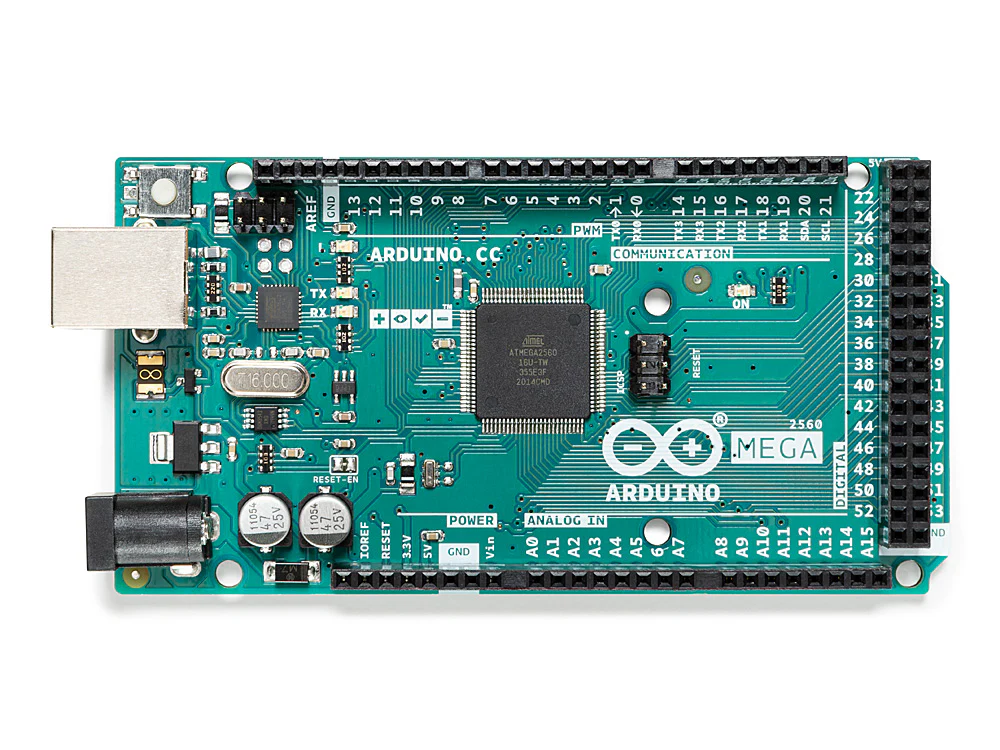
\includegraphics[width=0.4\textwidth]{figures/arduinomega.png}
    \caption{\textit{Arduino} Mega \cite{ArduinoMega}}
    \label{fig:arduinomega}
\end{figure}

No entanto, de forma a ultrapassar o problema levantado pelo elevado preço do \acrshort{labview}, surge um segundo objectivo que se prende com a substituição deste \textit{software} por outro que fosse gratuito e \textit{open source}. A eliminação do \acrshort{labview} implicou a implementação de um servidor. Sendo assim, numa primeira abordagem, foram analisadas algumas opções, tais como: \textit{FastApi}\footnote{\url{https://fastapi.tiangolo.com/}}, \textit{Django}\footnote{\url{https://www.djangoproject.com/}} e \textit{Flask}\footnote{\url{https://flask.palletsprojects.com/en/3.0.x/}}. Estas opções enquadram-se no que se pode chamar \textit{frameworks} ou \textit{micro-frameworks}. Neste caso são todas desenvolvidas para aplicação em \gls{python}.

Uma \textit{micro-framework} é um tipo de \textit{framework} minimalista, que fornece apenas as funcionalidades essenciais para o desenvolvimento de aplicações, sem incluir bibliotecas ou componentes adicionais que não os estritamente necessários. Isso permite a quem desenvolve adicionar apenas as funcionalidades específicas para cada projecto ou aplicação. Daqui resulta um ambiente de desenvolvimento mais leve e flexível \cite{Flask}.
Optou-se, então, pelo \textit{Flask} e as razões da escolha, assim como uma explicação mais detalhada serão apresentadas na Secção \ref{sec:arquitecturasoftware}.

É possível combinar o \gls{arduino} com o \gls{python}, mas isso implicaria uma mudança ao nível do \textit{firmware}, uma tarefa que não é trivial \cite{Arduinopython}. A linguagem nativa do \gls{arduino} é similar ao \textit{C++} e o \textit{firmware} instalado foi projectado para interpretar e executar código escrito nesse tipo de linguagem. De forma mais rigorosa, o uso do \textit{Python} no \gls{arduino} ou em qualquer outro microcontrolador, faz-se através de \textit{MicroPython}, uma implementação simples e eficiente do \gls{python} que inclui um pequeno subconjunto da bibliotecas padrão e é optimizado para funcionar em microcontroladores e em ambientes limitados \cite{MicroPythondefinition}. Quer isto dizer que todas as bibliotecas usadas na programação da aplicação ou projecto têm de ser carregadas para a memória dos microcontroladores. No caso do \gls{arduino} Mega, uma análise ao \textit{datasheet} \cite{megadatasheet} revela que este tem \SI{256}{Kbytes} reservados para o envio de programas e \SI{8}{Kbytes} de memória \textit{SRAM} reservado para variáveis temporárias.
Além destes problemas de memória e uma vez que é necessário que o \gls{arduino} funcione como servidor, foi necessário encontrar uma alternativa mais adequada Arduino Mega, versão apresentada na Figura \ref{fig:arduinomega} não é adequada.

No mercado, existe o \gls{ESP32}, uma alternativa mais poderosa que o \gls{arduino} e com placa de rede sem fios integrada, tal como é apresentado na Figura \ref{fig:ESP32}. No entanto, este microcontrolador sofre dos mesmos problemas de memória que o \gls{arduino} Mega e da utilização do \textit{MicroPython}. Uma análise ao \textit{datasheet} \cite{esp32datasheet} revela que a memória \textit{flash} varia entre os 4-16 \acrlong{mb}. No modelo ''ESP32-DEVKITC-32E``, que estava disponível para este projecto, o valor é de 4 \acrshort{mb} \cite{diferencaspython}. Estas limitações não permitem a implementação de um servidor minimamente robusto usando o \gls{arduino} Mega ou o \gls{ESP32}.

\begin{figure}[hbtp]
    \centering
    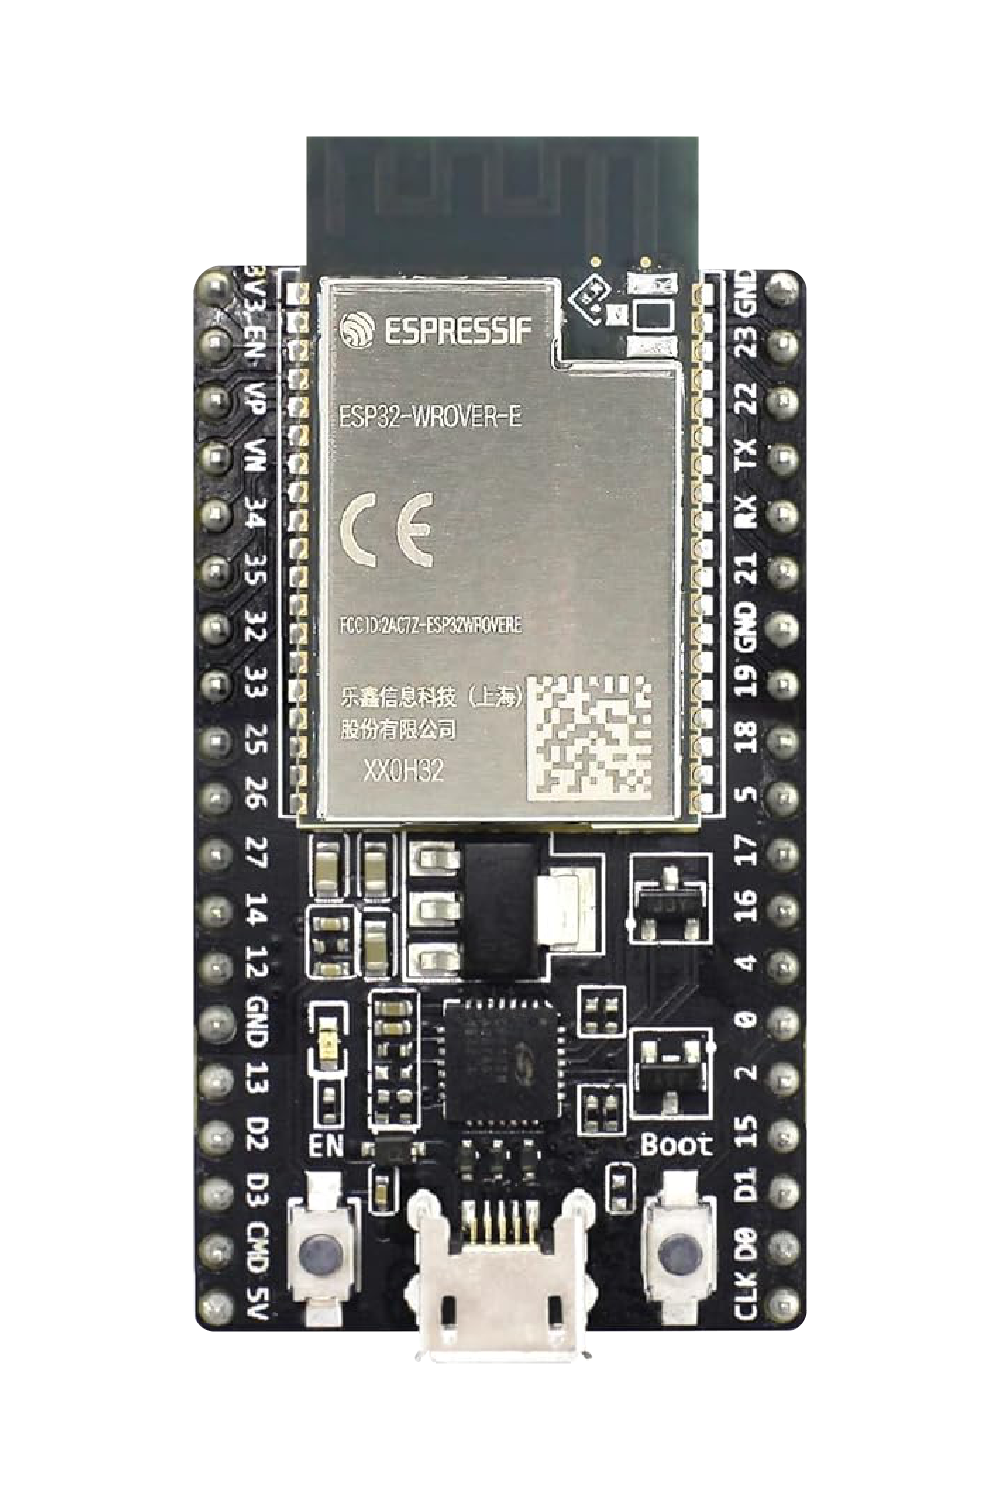
\includegraphics[width=0.4\textwidth]{figures/ESP32-DevKitC_L_0.png}
    \caption{\textit{ESP32} \cite{ESPDevKit}}
    \label{fig:ESP32}
\end{figure}

A opção seguinte recaiu no \gls{RaspberryPI}, versão 5\footnote{Doravante, sempre que for referido \textit{Raspberry Pi}, subentende-se a versão 5.}, que à data da escrita desta dissertação é a versão mais actual, apresentada na Figura \ref{fig:Raspberrypi5}. 

\begin{figure}[hbtp]
    \centering
    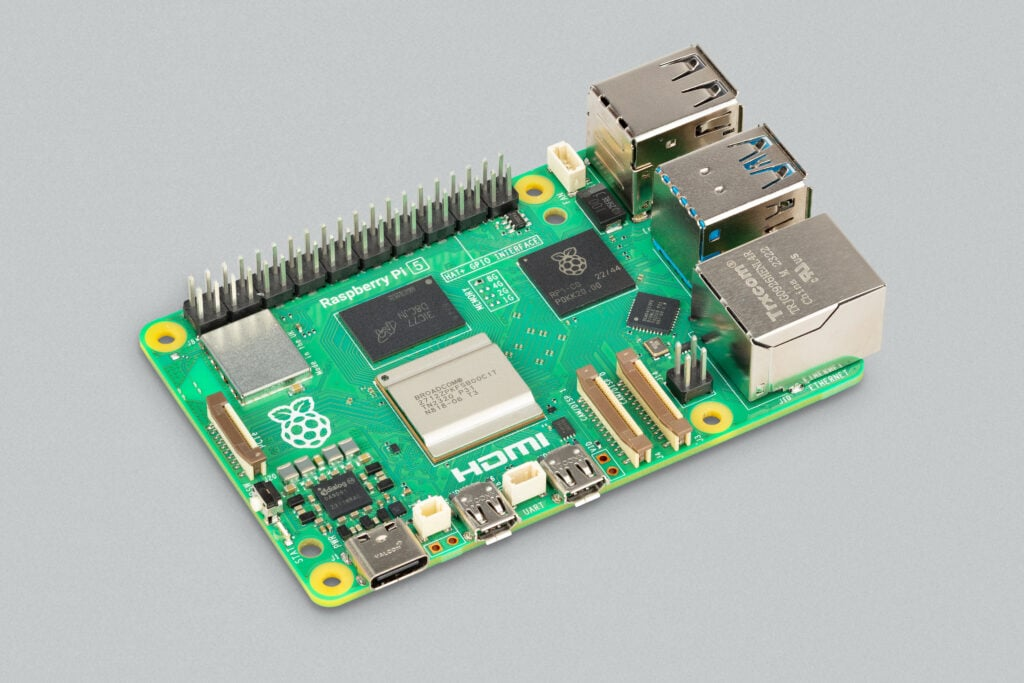
\includegraphics[width=0.4\textwidth]{figures/raspberrypi5.jpg}
    \caption{\textit{RaspberryPI5} \cite{introRaspberrypi5}}
    \label{fig:Raspberrypi5}
\end{figure}

Considerou-se, portanto, que seria uma mais-valia desenvolver um \acrshort{laboratório remoto} com as seguintes características:
\begin{itemize}
    \item \gls{python} como linguagem principal;
    \item \gls{RaspberryPI} como servidor \textit{Flask};
    \item \textit{Interface} com o utilizador desenvolvido em ~\acrfull{html}.
\end{itemize}

Estava dado o último passo na escolha do \textit{hardware} e do \textit{software} que viriam a compor o \acrshort{lare}.

\section{Solução proposta}
\label{sec:solucaoproposta}
Os objectivos principais foram apresentados na Secção \ref{sec:Objectivos} e as características gerais do projecto descritas na Secção \ref{sec:contextualização}. Pretende-se que o \acrshort{lare} seja um \acrshort{laboratório remoto} capaz de controlar e comandar um conjunto de experiências electrónicas, assim como efectuar medições de várias grandezas eléctricas. Para que a solução proposta seja completa e definitiva, é necessário definir os instrumentos de medida e os circuitos que compõem as experiências.

No contexto desta dissertação, o instrumento de medida adoptado foi o \acrfull{virtualbench}, modelo VB-8012 que pode ser controlado de duas formas: através do \textit{software} fornecido pela \acrshort{ni} ou através do \textit{pyVirtualBench}\footnote{Apesar de não ser abordado no contexto desta dissertação, existe também a possibilidade de aceder ao \acrshort{virtualbench} através do \acrshort{labview}.} \cite{AutomatingVB}. O \textit{pyVirtualBench} é um \gls{wrapper}\footnote{Este \gls{wrapper} é um \textit{software} de terceiros, suportado e mantido pela comunidade e não é diretamente suportado pela \acrshort{ni}.} que permite controlar o \acrshort{virtualbench} através de uma aplicação \gls{python} \cite{pyvirtualbench}. No entanto, este \gls{wrapper} não é compatível com \textit{Linux}.

Perante este facto, decidiu-se integrar um \acrshort{pc} no \acrshort{lare} - pormenores da instalação do \textit{driver} no \textit{site} da \acrshort{ni} \cite{AutomatingVB} - sendo que todo o peso computacional passaria para o \acrshort{pc} e o \gls{RaspberryPI} controlaria os relés. Esta decisão justifica-se pela possibilidade de, no futuro, o \textit{pyVirtualBench} vir a ser compatível com sistemas \textit{Linux}.

A outra forma de controlar o \acrshort{virtualbench} é usando a aplicação disponibilizada pela \acrshort{ni}  e compatível com \textit{Windows}. Esta aplicação faz uma apresentação integrada dos cinco instrumentos apresentados no \acrshort{virtualbench}, como pode ser visto na Figura \ref{fig:leituraohm}. A aplicação também inclui funcionalidades de fluxo de trabalho, como a importação e exportação de configurações de instrumentos e a captura de dados. Importa salientar que o \acrshort{virtualbench} não pode ser controlado simultaneamente por ambas as \textit{interfaces}.

\begin{figure}[hbtp]
    \centering
    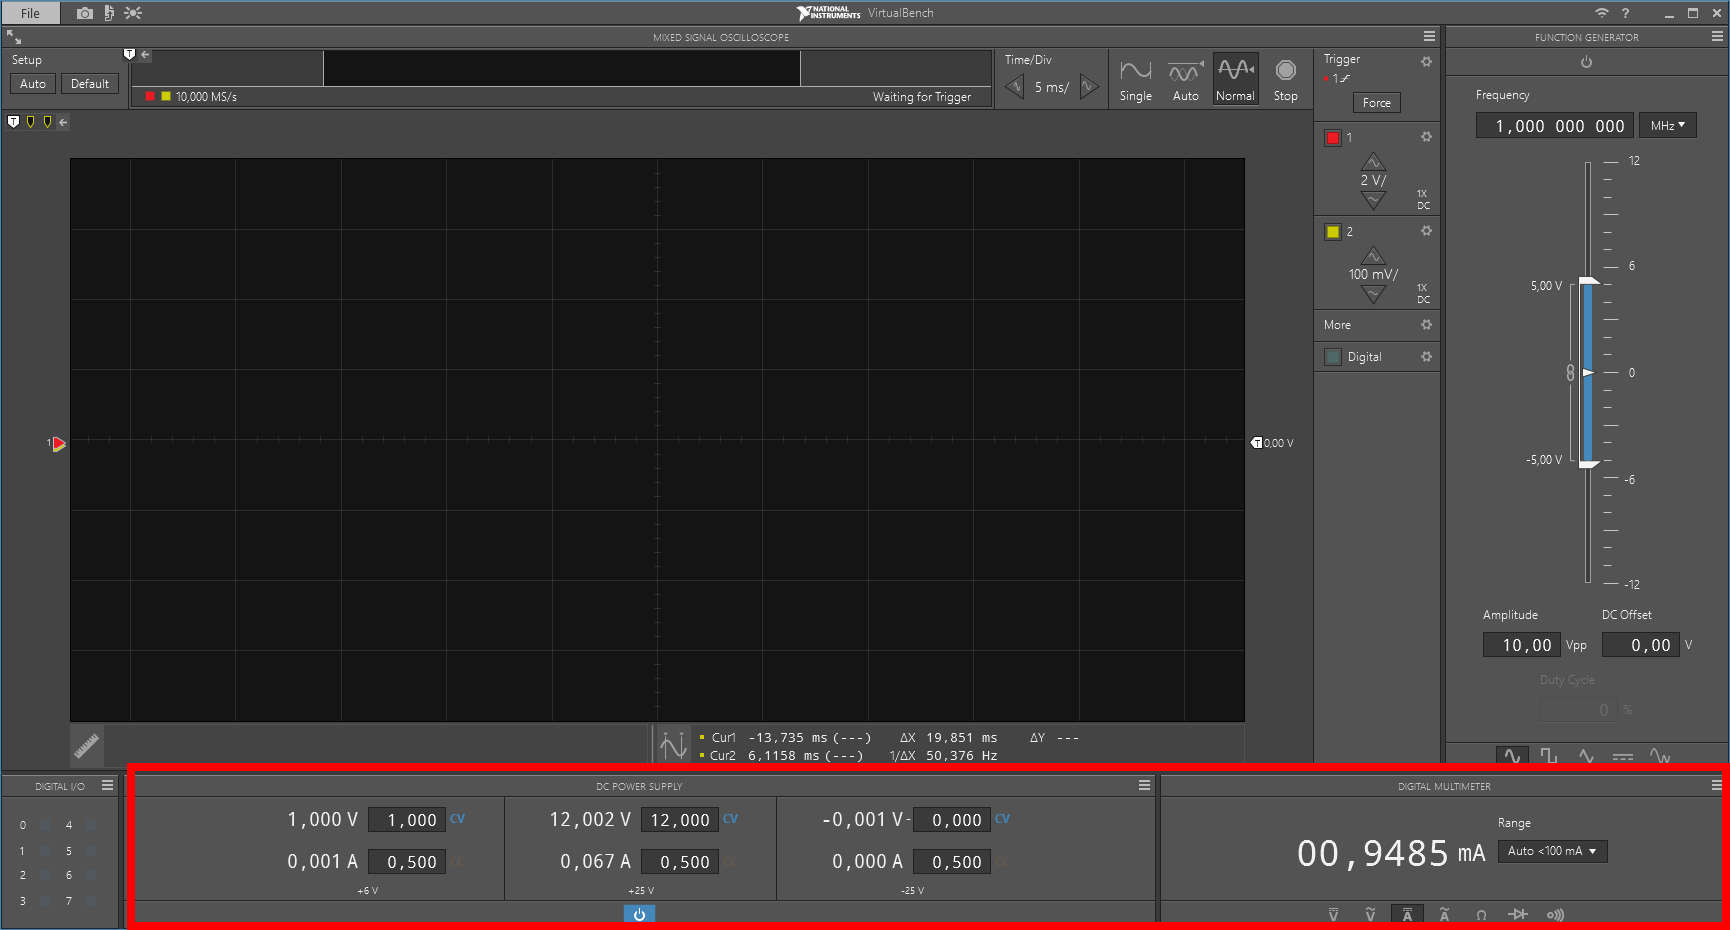
\includegraphics[width=0.7\textwidth]{figures/VB8012-OHM_Exemplo.png}
    \caption{Exemplo do \acrshort{virtualbench} usado como multímetro digital}
    \label{fig:leituraohm}
\end{figure}

As características do \acrshort{laboratório remoto} são as seguintes:
\begin{itemize}
    \item \gls{python} como linguagem principal;
    \item \acrshort{pc} como servidor \textit{Flask};
    \item \gls{RaspberryPI} como controlador dos relés;
    \item \textit{Interface} com o utilizador desenvolvido em \acrshort{html}.
\end{itemize}

Definidas - de uma forma geral - as soluções de \textit{hardware} e \textit{software}, agora com a integração de um \acrshort{pc} - passou-se ao estudo da arquitectura do \acrshort{lare}.

\section{Arquitectura}
\label{sec:arquitectura}
Como já se viu na Secção \ref{sec:contextualização}, a arquitectura do \acrshort{lare} proposta baseia-se numa estrutura cliente-servidor, suportada ao nível do \textit{hardware} pelo \acrshort{virtualbench}, pelo \gls{RaspberryPI} e um \acrshort{pc} como servidor. Uma representação geral do que será o \acrshort{lare} pode ser vista na Figura \ref{fig:representaçãogerallare}.

\begin{figure}[hbtp]
    \centering
    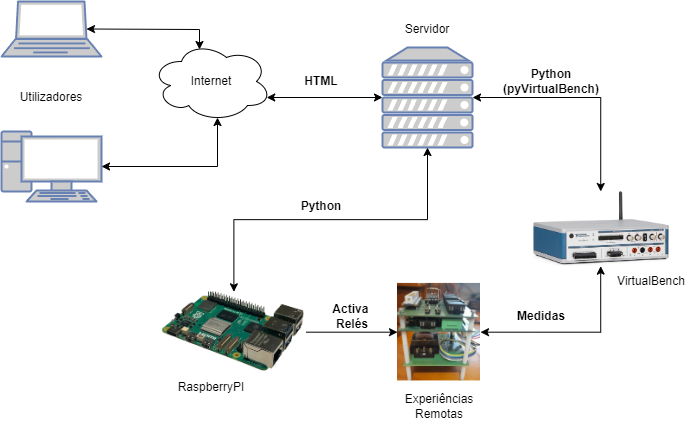
\includegraphics[width=0.7\textwidth]{figures/arquitectura_ver2.drawio.png}
    \caption{Arquitectura geral - \acrshort{lare}}
    \label{fig:representaçãogerallare}
\end{figure}

Antes de mais, importa clarificar as formas de comunicação entre os diversos dispositivos que compõem o \acrshort{lare}. Tanto o servidor, como o \gls{RaspberryPI} e o \acrshort{virtualbench} têm disponíveis interfaces de rede sem fios e com fios, assim como \textit{interfaces} \acrshort{usb}. A comunicação entre os diversos dispositivos é feita da seguinte forma:
\begin{itemize}
    \item \textbf{Servidor - \gls{RaspberryPI}}: comunicação via rede sem fios. Para maior flexibilidade e simplicidade de programação, a comunicação entre o servidor e o \gls{RaspberryPI} é feita através da rede sem fios, utilizando \textit{sockets} que, através da sua API, facilitam a comunicação entre processos em rede, independentemente da infra-estrutura utilizada — seja por ligação com fios, sem fios ou através de redes locais, permitindo, assim, o envio e recepção de mensagens entre dispositivos ligados em rede \cite{Sockets}. O fluxograma de uma chamada ao \textit{sockets} está representado na Figura \ref{fig:fluxogramasockets};
    \item \textbf{Servidor - \acrshort{virtualbench}}: comunicação via rede sem fios ou \acrshort{usb}. Entre estes dois dispositivos é, basicamente, indiferente a forma como é feita a comunicação. Isto porque esta parte é gerida pelos \textit{drivers} da aplicação instalada no \textit{Windows}. Independentemente de se utilizar o \textit{pyVirtualBench} ou a aplicação;
    \item \textbf{Controlo de relés e medidas}: O controlo dos relés é feito através da ligação directa do \gls{RaspberryPI} ao \textit{driver} dos relés. Por sua vez, as leituras e medições das grandezas eléctricas são efectuadas pelo \acrshort{virtualbench}, ligado directamente aos pontos específicos do circuito.
\end{itemize}

\begin{figure}[hbtp]
    \centering
    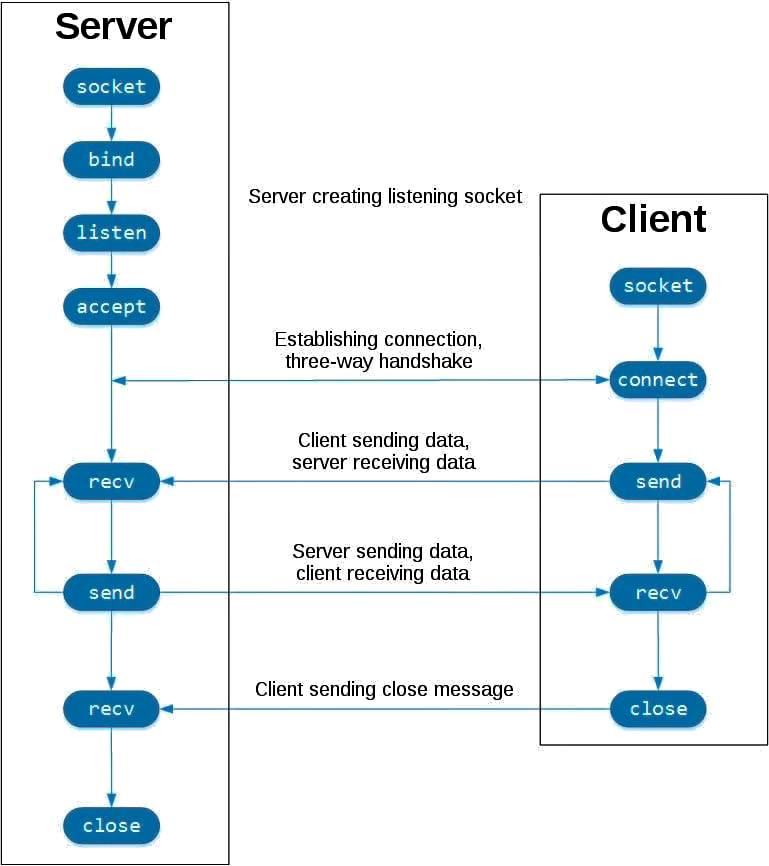
\includegraphics[width=0.5\textwidth]{figures/socketsdiagrama.png}
    \caption{Fluxograma de uma chamada ao \textit{socket} \cite{Sockets}}
    \label{fig:fluxogramasockets}
\end{figure}

Ao nível do \textit{software}, o servidor será implementado no \acrshort{pc} com base no \textit{Flask}, como já foi referido na Secção \ref{sec:contextualização} e \ref{sec:solucaoproposta}, e será descrito com mais pormenor na Secção \ref{sec:arquitecturasoftware}. A comunicação entre o servidor e o \acrshort{virtualbench}, entre o servidor e o \gls{RaspberryPI} e o controlo dos relés é feita em \textit{Python}. A \textit{interface} com o utilizador é feita em \acrshort{html}.

A Figura {\ref{fig:arquitecturalore}} apresenta com mais pormenor a solução implementada no \acrshort{lare}. De uma forma geral, podemos ver como é realizada a comunicação e a troca de informação entre os diferentes dispositivos de \textit{hardware}.

\begin{figure}[hbtp]
    \centering
    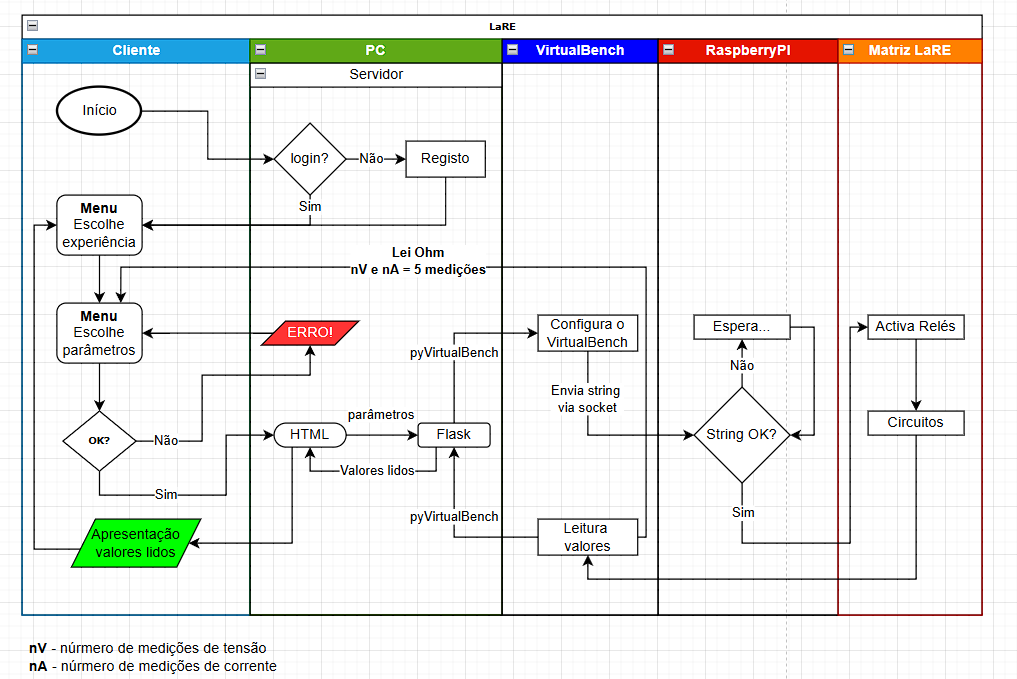
\includegraphics[width=0.7\textwidth]{figures/arquitectura_geral_LaRE.png}
    \caption{Arquitectura geral - \acrshort{lare} - \textbf{NOTE: Fig actualizada - opiniao PROF}}
    \label{fig:arquitecturalore}
\end{figure}

\section{Circuitos experimentais}
\label{sec:circuitos}
A escolha dos circuitos teve como base os que estão disponíveis no \acrshort{visir} do \acrshort{isep} e reduzindo os objectivos do \acrshort{lare} à sua forma mais básica, pode afirmar-se que se pretende ``provar um conceito''. Escolhendo experiências com circuitos integrados ou transístores, poderia tornar a implementação desnecessariamente mais complexa e, por conseguinte, com menos experiências. Portanto, o objectivo passará por criar um \acrshort{laboratório remoto} com experiências típicas para a introdução à electrónica e que permitam uma aprendizagem gradual em contexto de sala de aula. E, assim, ``provar o conceito''.

Sendo assim, os circuitos que compõem o \acrshort{lare} e satisfazem os critérios definidos em cima são:
\begin{itemize}
    \item Lei de Ohm;
    \item Rectificador de meia onda;
    \item Rectificador de onda completa;
    \item Filtro RC passa-baixo;
    \item Filtro RC passa-alto.
\end{itemize}

Doravante, considera-se que cada experiência é composta por dois circuitos distintos, com excepção da experiência dedicada à Lei de \textit{Ohm}. Por exemplo, a experiência sobre rectificação inclui os circuitos de meia onda e de onda completa; já a experiência dos filtros abrange os circuitos passa-baixo e passa-alto.

\subsection{Lei de \textit{Ohm}}
Na forma da Equação \ref{eq:leideohm}, a Lei de \textit{Ohm} estabelece que a resistência eléctrica ($R$) de um condutor é determinada pelo quociente entre a tensão elétrica ($U$) aplicada aos seus terminais e a corrente eléctrica ($I$) que o atravessa.  

\begin{equation} \label{eq:leideohm}
	R=\dfrac{U}{I}
\end{equation}

Isto significa que a Equação \ref{eq:leideohm} define uma relação linear entre a tensão e a corrente para uma determinada resistência de valor fixo, o que implica que o gráfico obtido, representado na Figura \ref{fig:graphohm}, é uma linha recta que passa pela origem. O declive dessa recta representa o valor da resistência elétrica ($R$). A Lei de \textit{Ohm} é descrita com maior detalhe no Capítulo~2 da 10.\textsuperscript{a} edição de Hayt \textit{et al.}~\cite{hayt}.

\begin{figure}[hbtp]
	\centering
	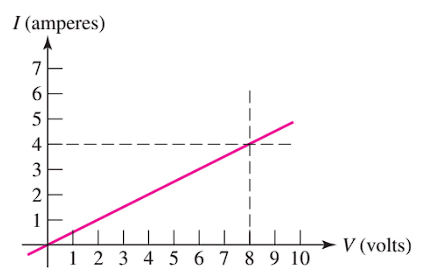
\includegraphics[width=0.4\textwidth]{figures/grafico_Ohm.png}
	\caption{Gráfico da Lei de \textit{Ohm}\cite{hayt}}
	\label{fig:graphohm}
\end{figure}

Da forma como foi implementado, há duas possibilidades de realizar este estudo, exemplificado nas Figuras \ref{fig:Opção_1} e \ref{fig:Opção_2}. O tutor ou professor, poderá optar por apresentar o conceito de duas formas distintas, em ambos os casos são efectuadas cinco medições, construido o respectivo gráfico e calculado o valor do declive da recta analiticamente. A diferença está na forma como se confrontam os resultados práticos. No entanto, no contexto desta dissertação foi  implementado o caso descrito na Figura \ref{fig:Opção_1}\footnote{Como trabalho futuro, o menu poderia ser desenvolvido para o utilizador, aluno ou professor escolher a opção pretendida.}. 

\begin{figure}[hbtp]
	\centering%
		\centering
		\subfloat[\centering Opção 1\label{fig:Opção_1}]{{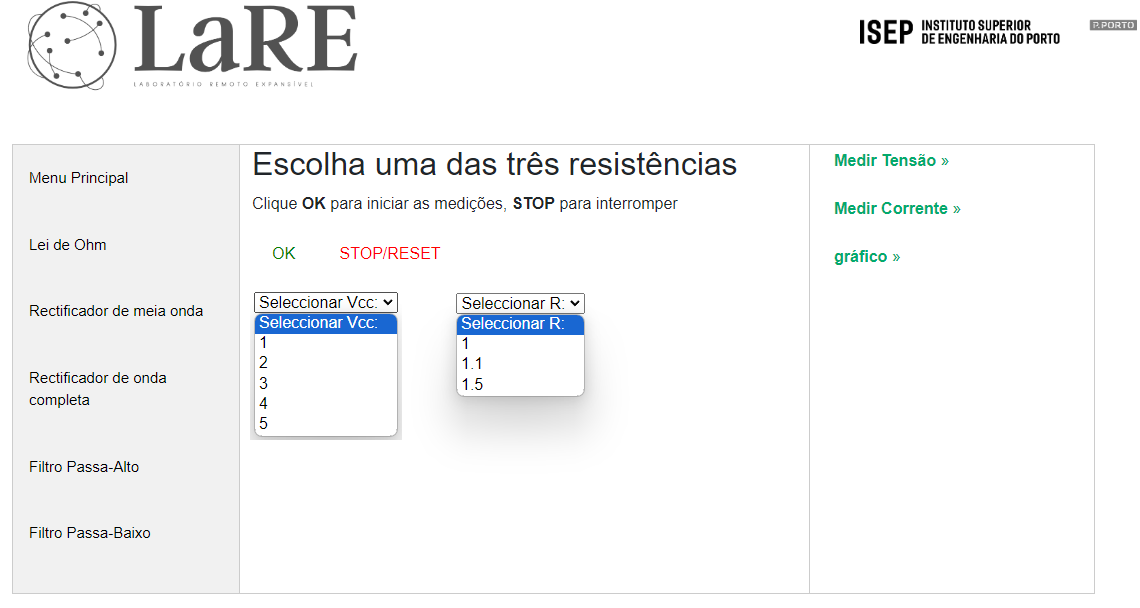
\includegraphics[width=6.3cm]{figures/ohm_escolha.png} }}%
		\qquad
		\subfloat[\centering Opção 2\label{fig:Opção_2}]{{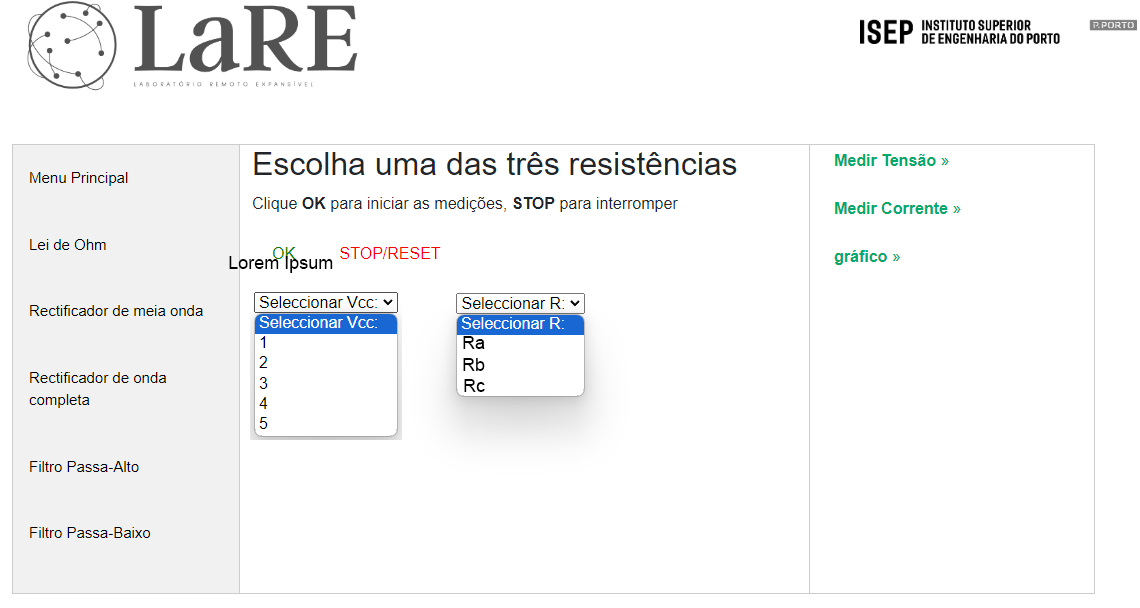
\includegraphics[width=6.3cm]{figures/ohm_escolha_abc.png} }}%
		\caption{Experiência Lei de \textit{Ohm}}%
		\label{fig:experienciaOHM}%
	\end{figure}

No caso em que a resistência é dada, o declive pode ser calculado e confrontado com as soluções, sendo que no caso em que é desconhecida, o declive da recta é calculado e a partir deste do resultado infere-se o valor da resistência. 

\subsection{Rectificadores}
\label{sec:circuitosrectificadores}
Nas experiências dos rectificadores pretende-se estudar e avaliar a diferença entre os dois tipos de rectificação, consoante as quatro combinações possíveis dos pares resistência/condensador e a influência que têm na variação da tensão de \textit{ripple}. No caso da rectificação de meia onda, é ainda possível variar a frequência entre os \SI{50}{\hertz} e \SI{2000}{\hertz} mas no caso da rectificação de onda completa, a frequência é fixa ao valor da rede eléctrica - \SI{50}{\hertz}.

A Figura~\ref{fig:blocosrectificacao} apresenta o diagrama de blocos simplificado do processo de rectificação, que pode ser usado, por exemplo, para o projecto duma fonte de alimentação em contexto de sala de aula. Este é composto por quatro blocos principais:

\begin{itemize}
    \item Bloco 1 - Transformador: reduz a tensão proveniente da rede eléctrica para valores mais baixos e adequada ao nível de tensão alternada que se deseja;
    \item Bloco 2 - Rectificação: realiza a conversão da tensão alternada \acrshort{ca} em tensão contínua unidirecional, ainda com ondulação;
    \item Bloco 3 - Filtragem: responsável pela suavização da forma de onda, reduzindo a componente alternada (\textit{ripple});
    \item Bloco 4 - Estabilização:  regula e estabiliza a tensão de saída, garantindo um valor contínuo e constante.
\end{itemize}

\begin{figure}[hbtp]
	\centering
	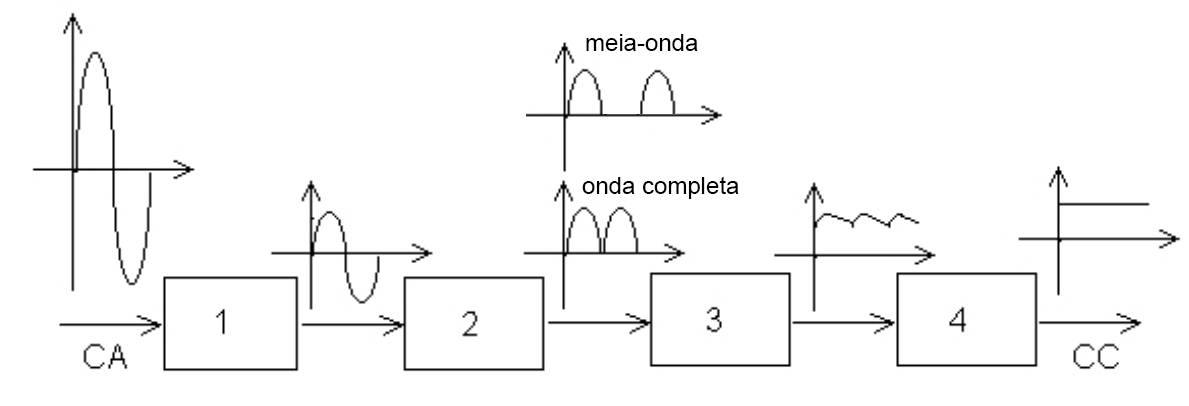
\includegraphics[width=0.7\textwidth]{figures/diagramablocosrectificacao.png}
	\caption{Diagrama de blocos da rectificação \cite{sedrasmith}}
	\label{fig:blocosrectificacao}
\end{figure}

A tensão de \textit{ripple} é uma componente variável no tempo que surge à saída do Bloco 3 - Filtragem -  devendo esta ser minimizada para estabilizar a tensão de saída em corrente contínua - Bloco 4 - tal como ilustrado na Figura~\ref{fig:blocosrectificacao}. As Figuras~\ref{fig:formadeonda_MO} e \ref{fig:esquemaMO} representam, com mais pormenor, a forma de onda à saída do Bloco 3 quando é utilizada a rectificação de meia onda, considerando um díodo ideal. Estes circuitos e a respectiva fundamentação teórica são descritos com maior detalhe no Capítulo~4 da 8.\textsuperscript{a} edição de Sedra \textit{et al.}~\cite{sedrasmith}, de onde foram adaptados.

\begin{figure}[hbtp]
	\centering%
		\centering
		\subfloat[\centering Forma de onda à saída do Bloco 3\label{fig:formadeonda_MO}]{{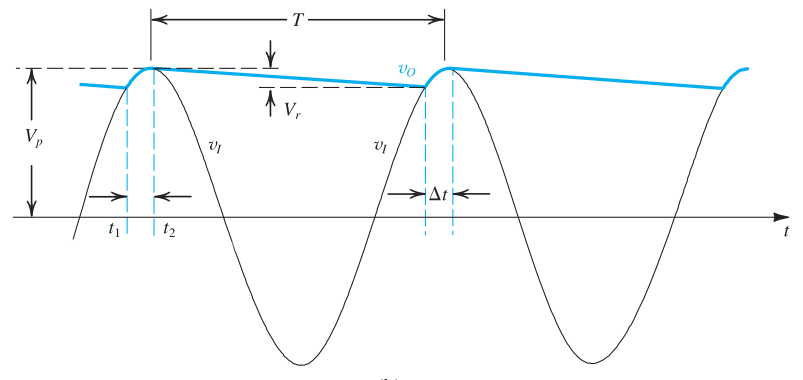
\includegraphics[width=6cm]{figures/sedra_ripple.png} }}%
		\qquad
		\subfloat[\centering Esquema rectificador \label{fig:esquemaMO}]{{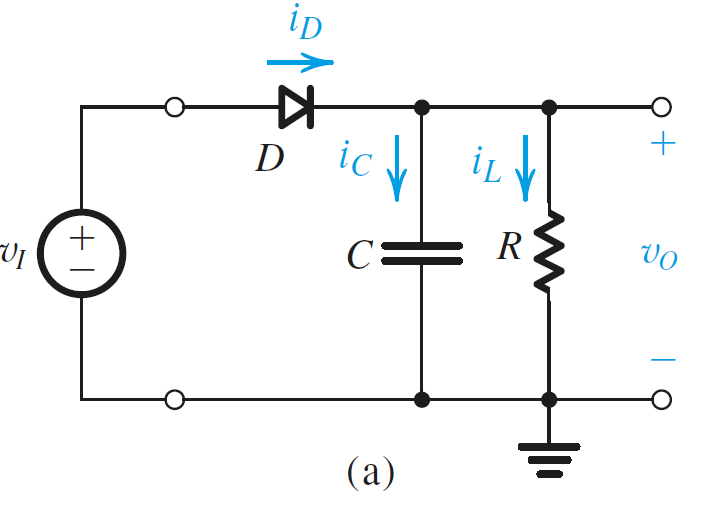
\includegraphics[width=5cm]{figures/meia_onda_Sedra.png} }}%
		\caption{Rectificação meia onda \cite{sedrasmith}}%
		\label{fig:rectificacaomeiaonda}%
\end{figure}

A tensão de \textit{ripple} pode ser calculada através da Equação \ref{eq:vripplecompleta}:

\begin{equation} \label{eq:vripplecompleta}
	U_{r} = U_{P}(1-e^{-\frac{T}{RC}})
\end{equation}

Observa-se, a partir da Equação \ref{eq:vripplecompleta}, que quando a constante de tempo $RC >> T$, o cálculo da tensão de \textit{ripple} pode ser reduzido à Equação \ref{eq:vripple}.

\begin{equation} \label{eq:vripple}
	U_{r} = \frac{U_{P}}{fRC}
\end{equation}

Sendo que, neste caso, a tensão de \textit{ripple} é baixa e $v_{o}$, ou seja, a tensão à saída do filtro é practicamente constante e dada pela Equação \ref{eq:tensaosaida}:

\begin{equation} \label{eq:tensaosaida}
	u_{o} = U_{P} - \dfrac{1}{2}U_{r}	
\end{equation}

No entanto, pode tornar-se este circuito mais eficiente se se usar a rectificação de onda completa. A Figura~\ref{fig:formadeonda_OC} e a Figura~\ref{fig:esquemaOC} representam a forma de onda (... que como se pode ver a frequência do \textit{ripple} é o dobro da frequência da onda de entrada.) e o esquema, tal como descritos com maior detalhe no Capítulo~4 da 8.\textsuperscript{a} edição de Sedra \textit{et al.}~\cite{sedrasmith}, de onde foram também adaptados. 

\begin{figure}[hbtp]
	\centering%
		\centering
		\subfloat[\centering Forma de onda à saída do Bloco 3\label{fig:formadeonda_OC}]{{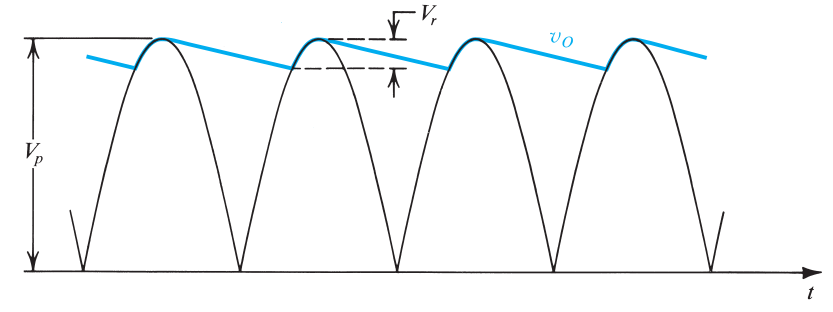
\includegraphics[width=6cm]{figures/sedra_ripple_OC.png} }}%
		\qquad
		\subfloat[\centering Esquema rectificador \label{fig:esquemaOC}]{{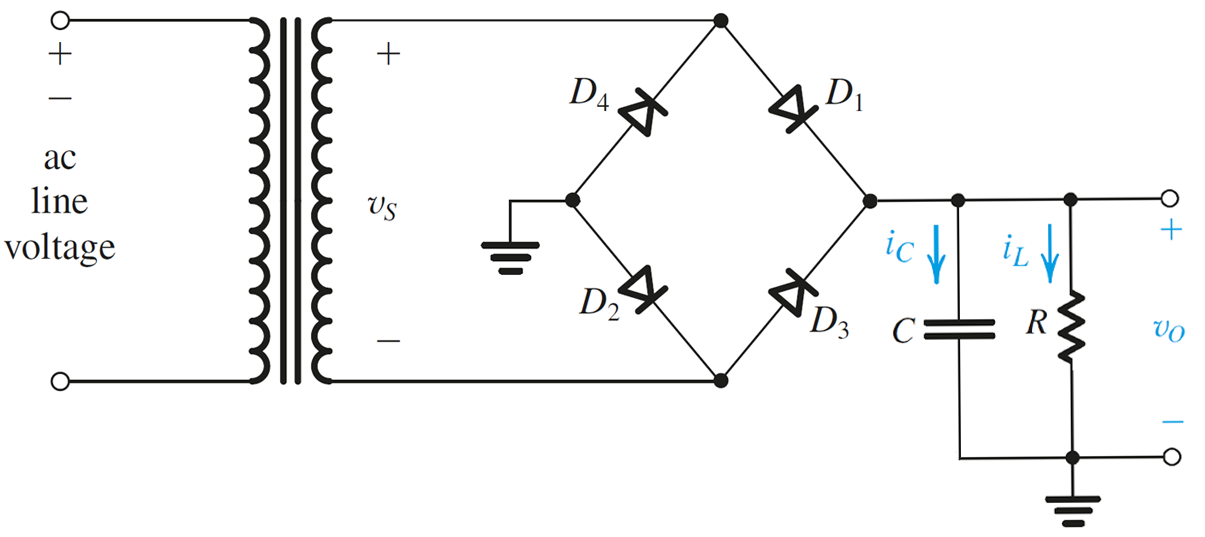
\includegraphics[width=5cm]{figures/onda_completa_Sedra.png} }}%
		\caption{Rectificação onda completa \cite{sedrasmith}}%
		\label{fig:rectificacaomeiaonda}%
\end{figure}

Sendo assim, o valor da tensão de \textit{ripple}, neste caso, será dado pela Equação \ref{eq:vrippleOC}:

\begin{equation} \label{eq:vrippleOC}
	U_{r} = \frac{U_{P}}{2fRC}
\end{equation}

São estas formas de onda, representadas pelas Figuras \ref{fig:formadeonda_MO} e \ref{fig:sedraripplecompleta}, que se pretendem estudar e avaliar, assim como os valores dados pelas Equações \ref{eq:vripple} e \ref{eq:vrippleOC}. (A Equação \ref{eq:vripplecompleta} deve ser usada quando os valores dos condensadores e resistências são pequenos ou frequência é baixa, isto é, quando o \textit{ripple} não é desprezável.)

\subsection{Filtros}
Representados na Figura \ref{fig:filtrosesqgeral} estão os filtros simplificados, leccionados em contexto de sala de aula no ensino secundário. Estes circuitos são descritos com maior detalhe no Capítulo~17 da 8.\textsuperscript{a} edição de Sedra \textit{et al.}~\cite{sedrasmith}, de onde foram adaptados.

\begin{figure}[hbtp]
	\centering%
		\centering
		\subfloat[\centering Filtro passa-baixo\label{fig:filtro_pb}]{{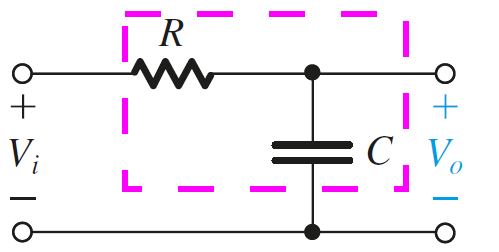
\includegraphics[width=6cm]{figures/Sedra_FPB_GIMP.png} }}%
		\qquad
		\subfloat[\centering Filtro passa-alto\label{fig:filtro_pa}]{{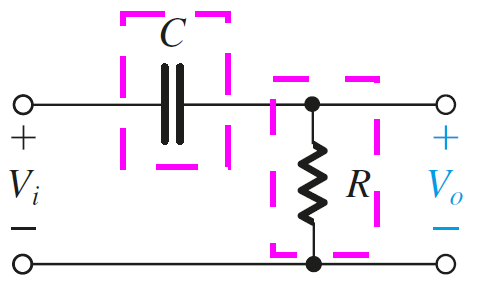
\includegraphics[width=6cm]{figures/Sedra_FPA_GIMP.png} }}%
		\caption{Esquemas dos filtros \cite{sedrasmith}}%
		\label{fig:filtrosesqgeral}%
\end{figure}

A possibilidade de variar a frequência do sinal de entrada permite que estas experiências sejam utilizadas para estudar a resposta em frequência dos filtros, analisar o Diagrama de \textit{Bode}, determinar a frequência de corte dada pela Equação \ref{eq:frequenciacorte} e ainda relacionar, por exemplo, o valor da tensão de entrada com a tensão de saída. 

\begin{equation} \label{eq:frequenciacorte}
	f_{c} = \frac{1}{2\pi RC}
\end{equation}

As Figuras \ref{fig:Bode_pb} e \ref{fig:Bode_pa} apresentam os Diagramas de \textit{Bode} \textins{ideais}, que servem de referência para o estudo desta experiência. 

\begin{figure}[hbtp]
	\centering%
		\centering
		\subfloat[\centering Filtro passa-baixo\label{fig:Bode_pb}]{{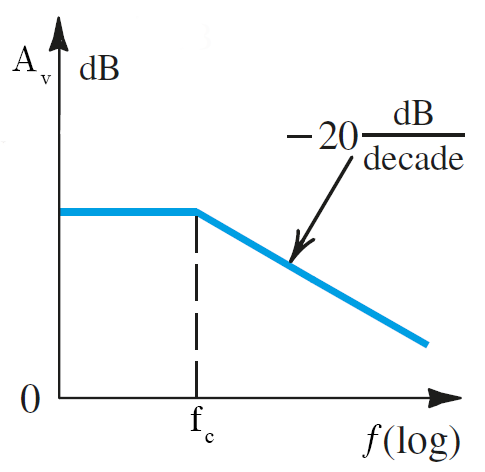
\includegraphics[width=6cm]{figures/Sedra_BodeFPB.png} }}%
		\qquad
		\subfloat[\centering Filtro passa-alto\label{fig:Bode_pa}]{{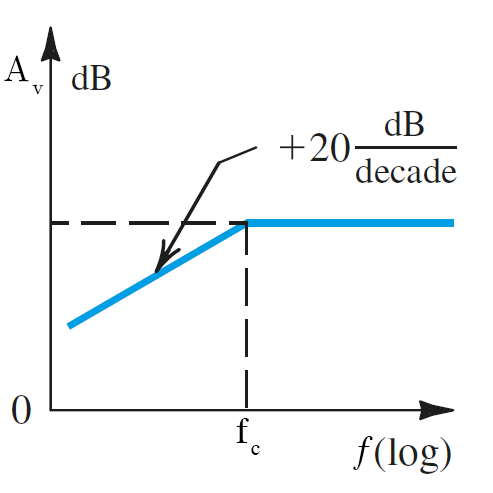
\includegraphics[width=6cm]{figures/Sedra_BodeFPA.png} }}%
		\caption{Diagramas de \textit{Bode} \textins{ideal} \cite{sedrasmith}}%
		\label{fig:Bodeesqgeral}%
\end{figure}

	Para além da análise em frequência, um outro aspeto complementar a considerar é a relação entre as ondas de entrada e saída, em função da frequência. Nos filtros, o intervalo de frequências permitido é igual ao já referido para os rectificadores: entre \SI{50}{\hertz} a \SI{80000}{\hertz}. 
	
	A frequência de corte de um filtro é definida como o ponto onde o ganho do filtro sofre uma atenuação de \SI{3}{\decibel} em relação ao seu valor máximo. 	Para um filtro passa-baixo (passa-alto) ideal, o ganho em baixas (altas) frequências é unitário. Quando o sinal atinge a frequência de corte, a relação entre a tensão de saída e a tensão de entrada reduz-se para:  
	
	\begin{equation} \label{eq:relacaoGanho}
		\frac{U_{out}}{U_{in}} = \frac{1}{\sqrt{2}} \approx 0.707
	\end{equation}
	
	\ldots ou na escala logarítmica:  
\begin{equation} \label{eq:relacaoGanhodB}
	\frac{U_{out}}{U_{in}} = 20 \log_{10} (0.707) \approx -\SI{3}{\decibel}	
\end{equation}
	
Assim, a frequência de corte de um filtro corresponde ao ponto em que a amplitude do sinal de saída é aproximadamente $70.7\%$ da amplitude do sinal de entrada, o que corresponde a -\SI{3}{\decibel}. 

\section{Hardware}
\label{sec:hardware}
\subsection{VirtualBench}
Este dispositivo desenvolvido pela \acrshort{ni} integra vários instrumentos e ferramentas de teste, tais como um osciloscópio digital com análise de protocolo, um gerador de formas de onda, um multímetro digital, uma fonte de alimentação \acrfull{cc} programável e E/S digitais num único dispositivo que se liga a um \acrshort{pc}, via \acrshort{usb} ou rede sem fios, como se pode ver na Figura \ref{fig:paineltraseiro}. As principais características deste modelo estão descritas na Figura \ref{fig:paineldianteiro} \cite{datasheetVirtualBench}. A forma como pode ser controlado e configurado já foi abordada na Secção \ref{sec:solucaoproposta}.

\begin{figure}[hbtp]
    \centering
    \centering
    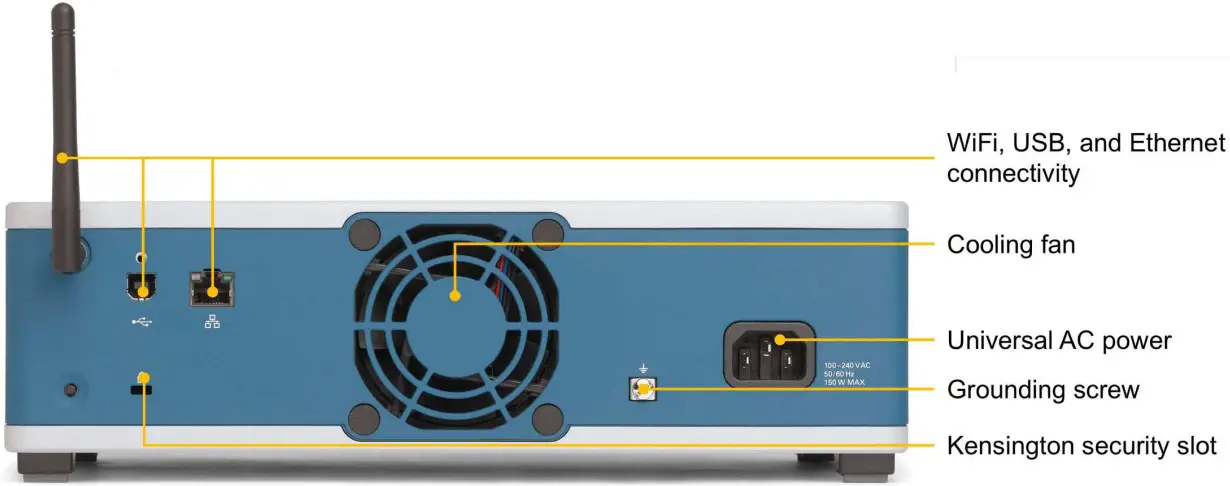
\includegraphics[width=0.5\textwidth]{figures/virtualbench_back-panel.jpg}
    \caption{Painel traseiro \textit{VirtualBench} VB-8012  \cite{datasheetVirtualBench}.}
    \label{fig:paineltraseiro}
\end{figure}

\begin{figure}[hbtp]
    \centering
    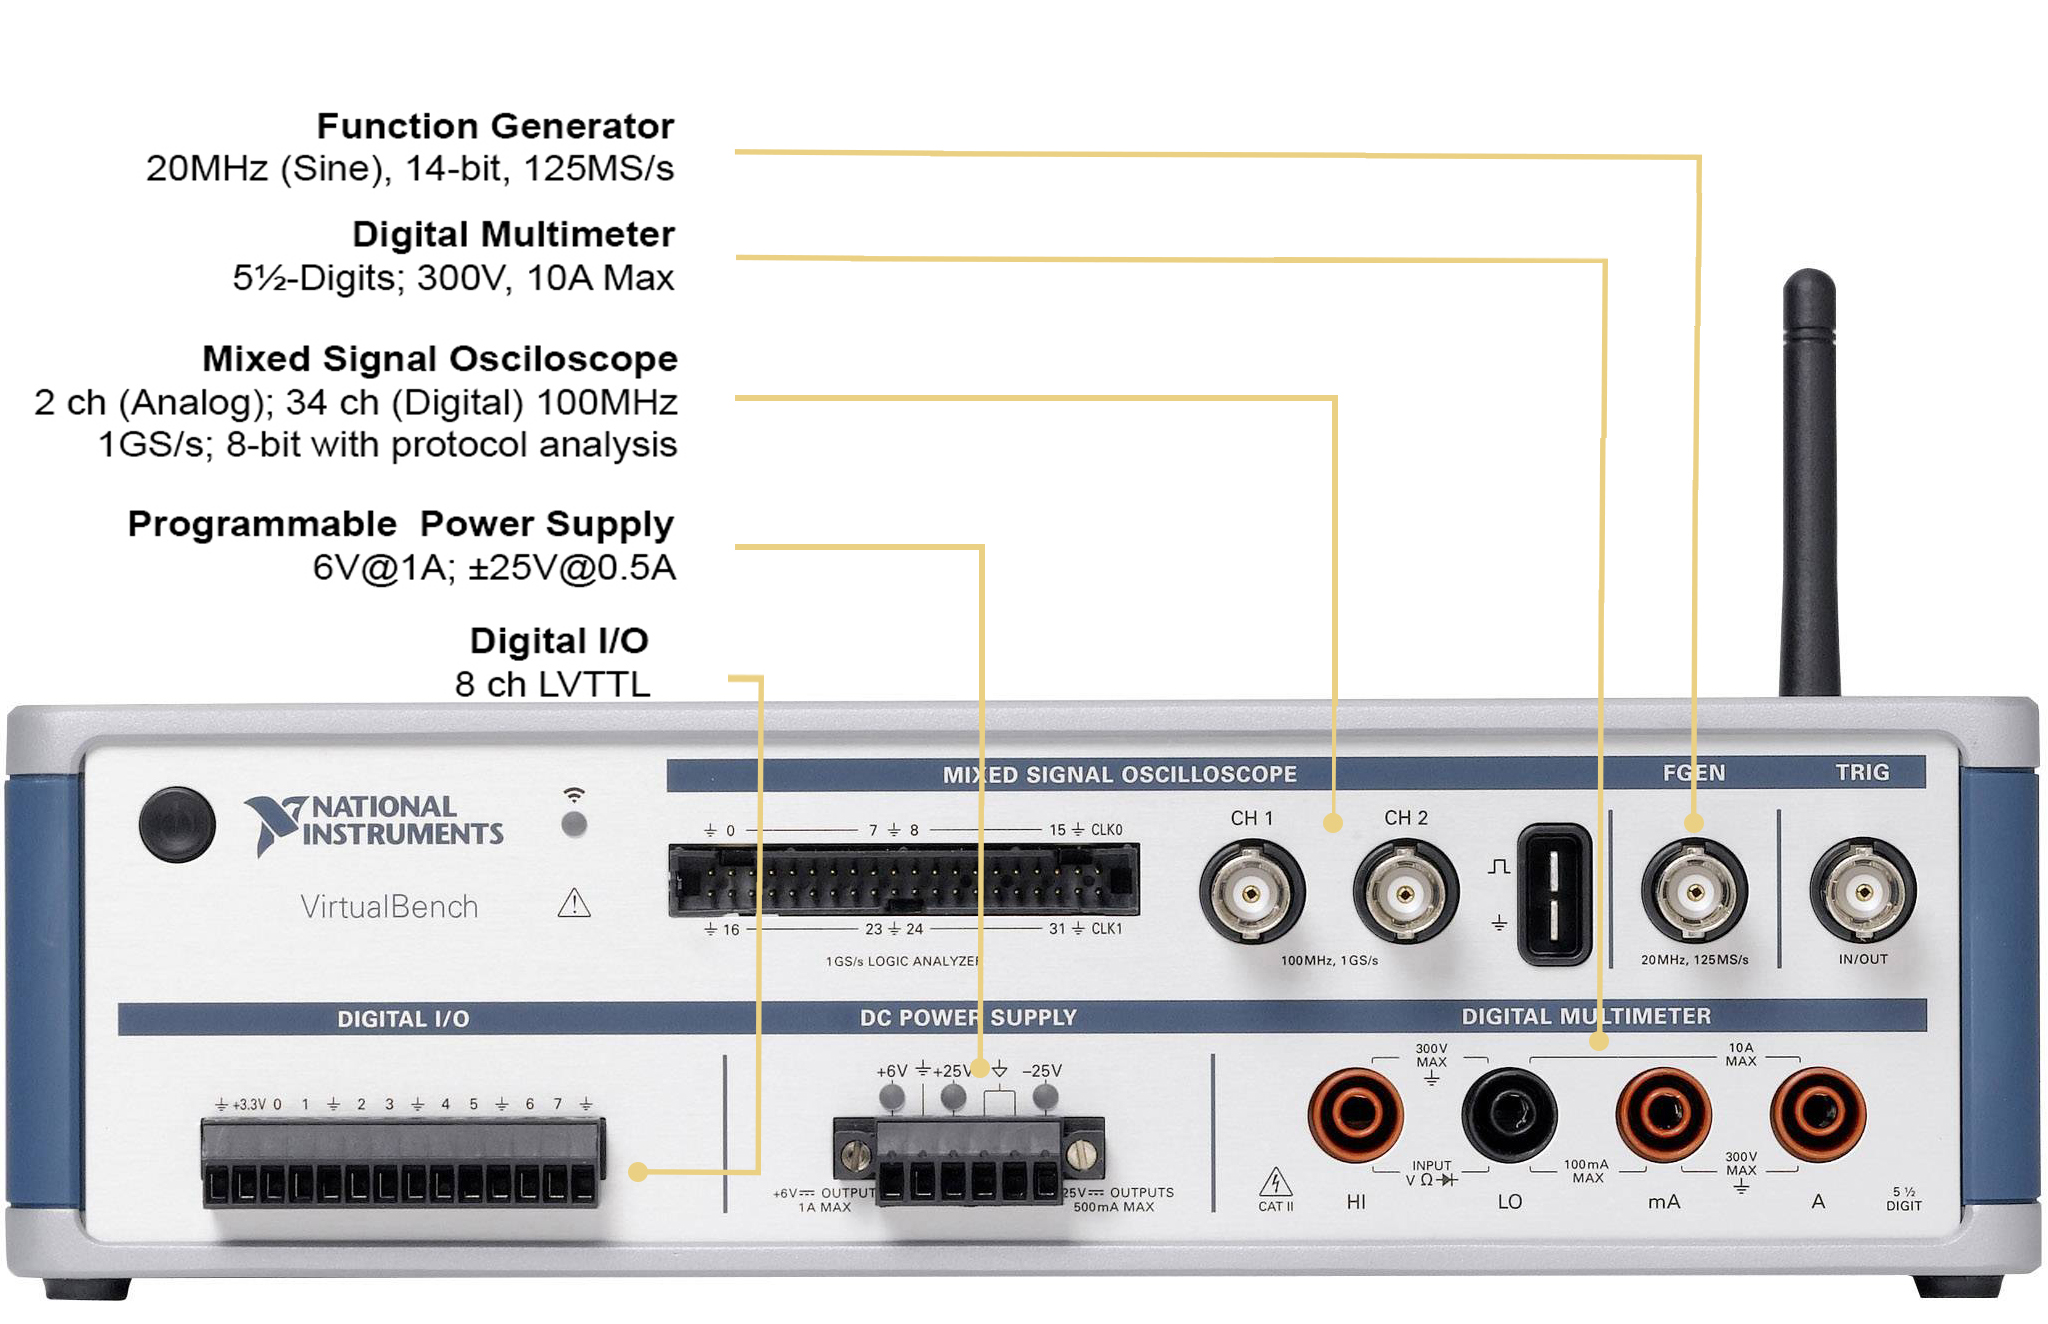
\includegraphics[width=0.5\textwidth]{figures/virtualbench_front-panel.jpg}
    \caption{Painel frontal \textit{VirtualBench} VB-8012  \cite{datasheetVirtualBench}.}
    \label{fig:paineldianteiro}
\end{figure}

\subsection{Matriz LaRE}
\label{sec:matriz}
Definidas as soluções de \textit{hardware} e \textit{software}, bem como as experiências a implementar, iniciou-se o projecto da matriz. Tal como anteriormente, e tendo o \acrshort{visir} como referência, decidiu-se desenvolver uma matriz cujas placas respeitem as dimensões definidas pelo consórcio \gls{pc/104} \cite{PC104}, o qual estabelece um padrão caracterizado pelo seu formato compacto e modular.

Os esquemas finais das experiências encontram-se no Anexo \ref{AppendixA}, onde se pode verificar que o número de relés necessários varia entre 8 — no caso da Lei de \textit{Ohm} — e 13 — nos casos dos rectificadores e dos filtros. Sendo assim, com o objectivo de facilitar a implementação, os testes, a detecção de erros e, mais tarde, a manutenção, optou-se por dividir o \acrshort{lare} em três placas. O desenho dos esquemas e dos \acrfull{pcb} foram elaborados com recurso ao \gls{kicad}. A Figura \ref{fig:matrizlare} apresenta uma visão geral da matriz do \acrshort{lare}. 

\begin{figure}[hbtp]
	\centering
	\includegraphics[width=0.4\textwidth]{figures/lare_3placas.png}
	\caption{Matriz do \acrshort{lare}}
	\label{fig:matrizlare}
\end{figure}

\subsubsection{Lei de \textit{Ohm}}
A placa desenvolvida para esta experiência está representada na Figura \ref{fig:placaleideohm}:

\begin{figure}[hbtp]
	\centering
	\includegraphics[width=0.5\textwidth]{figures/lare_ohm_BLOCOS.png}
	\caption{\textins{Placa} Lei de \textit{Ohm}}
	\label{fig:placaleideohm}
\end{figure}

\begin{enumerate}
	\item Ligação ao \gls{RaspberryPI} através de um conector \acrfull{idc} de 40 pinos (1);
	\item Relés (2);
	\item Ligações aos aparelhos de medida (3);
	\item \textit{Drivers} de relés e registo de deslocamento (4);
	\item Resistências em estudo (5);
	\item Ligação à placa seguinte através de conectores ``Arduino stackable'' (6).
\end{enumerate}

\subsubsection{Rectificadores/Filtros}
A Figura \ref{fig:placarectificadores} apresenta a placa da experiência referente aos rectificadores/filtros:

\begin{figure}[hbtp]
	\centering
	\includegraphics[width=0.5\textwidth]{figures/lare_rectificador_filtros_BLOCOS.png}
	\caption{\textins{Placa} rectificadores e filtros}
	\label{fig:placarectificadores}
\end{figure}
 
\begin{enumerate}
	\item Rectificação;
		\begin{enumerate}
			\item \label{diodos}Díodo rectificador - meia onda ($1_{a}$) e Ponte rectificadora - onda completa ($1_{b}$);	
		\end{enumerate}
    \item Relés (2);
    \item Resistências - \textins{componentes comuns a ambas as experiência}(3);
  	\item \textit{Drivers} de relés e registo de deslocamento (4);
	\item Condensadores \textins{componentes comuns a ambas as experiências}(5);
	\item Ligação à placa seguinte através de conectores ``Arduino stackable'' (6);
	\item Resistência e condensador exclusivo dos filtros (7).
\end{enumerate}

\subsubsection{Fontes de alimentação}
A placa referente às fontes de alimentação está representada na Figura~\ref{fig:placartransformador}. É constituída por um transformador de \SI{230}{\volt}/\SI{8}{\volt}CA, uma ponte rectificadora que realiza a rectificação de onda completa e uma fonte de \SI{5}{\volt}, regulada com o \textit{LM317}\cite{LM317}. O esquema completo encontra-se disponível no Anexo~\ref{AppendixA}.

\begin{figure}[hbtp]
	\centering
	\includegraphics[width=0.3\textwidth]{figures//lore_fonte.jpg}
	\caption{\textins{Placa} fontes de alimentação}
	\label{fig:placartransformador}
\end{figure}

\begin{comment}
\begin{figure}[hbtp]
    \centering
    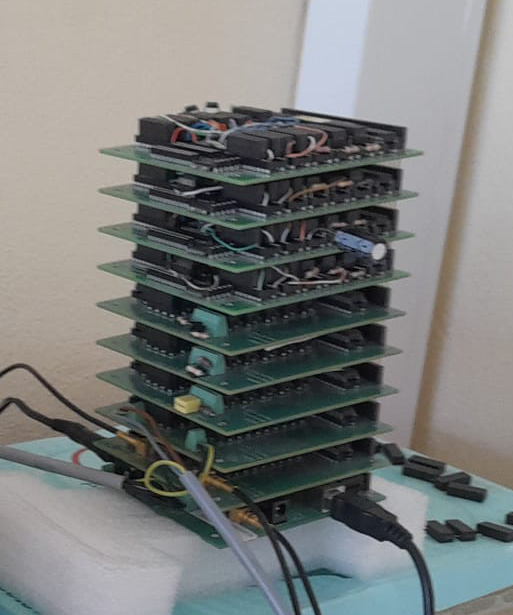
\includegraphics[width=0.3\textwidth]{figures/promenorvisirISEP.png}
    \caption{Placas PC/104 do \acrshort{visir} - \acrshort{isep} - \textbf{Foto com melhor qualidade}}
    \label{fig:visir104}
\end{figure}
\end{comment}

\subsection{Raspberry Pi}
\label{sec:RaspberryPI}
Como já foi referido na Secção \ref{sec:contextualização}, a ideia inicial passava por utilizar o \gls{RaspberryPI} como servidor e como controlador dos relés, no fundo desempenhando as funções de \acrshort{rlms}. Este dispositivo insere-se numa gama de pequenos computadores de placa única \gls{sbc}, acessíveis e versáteis, como o \textit{Banana Pi}, \textit{BeagleBone Black}, \textit{Orange Pi} ou \textit{Odroid}, amplamente utilizados em ensino, prototipagem e aplicações de \acrshort{iot}. 

Em contexto de laboratório estavam disponíveis os modelos PI2 e PI3, algo desactualizados. O PI3 já se mostrou lento nos primeiros testes e, por isso, optou-se pela última versão do \gls{RaspberryPI}, que à data da escrita deste documento é a 5. Esta versão traz várias melhorias e novos recursos, sendo que as principais diferenças de \textit{hardware} para a versão 4B estão representadas na Tabela \ref{Table:diferencasPI4PI5}. No entanto, estas melhorias acarretam um maior consumo de energia e, por isso, é recomendado o uso de arrefecimento activo \cite{Raspberrytech}. Na Figura \ref{fig:pi5dissipador} está representado o \gls{RaspberryPI} usado no \acrshort{lare}.

\begin{figure}[hbtp]
    \centering
    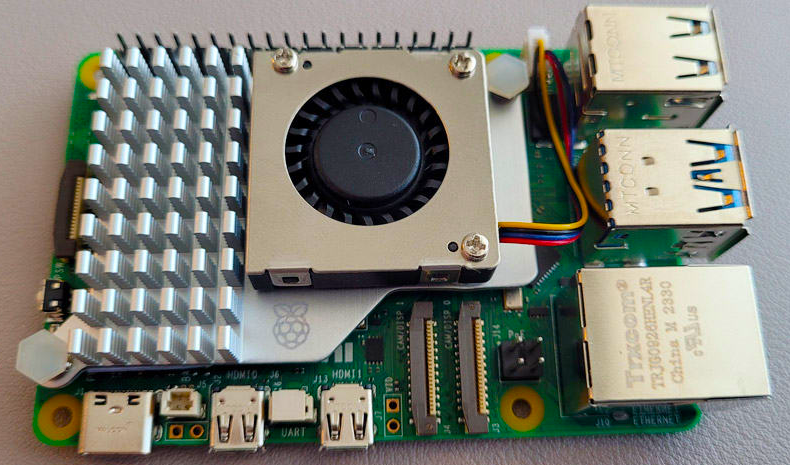
\includegraphics[width=0.5\textwidth]{figures/pi5_dissipador.png}
    \caption{\textit{Raspberry PI5} com dissipador activo utilizado no \acrshort{lare}}
    \label{fig:pi5dissipador}
\end{figure}

\begin{table}[htb]
    \centering
    \caption{Raspberry PI4 \textit{vs Raspberry PI5 - principais diferenças} \cite{Raspberrypi5}}
    \label{Table:diferencasPI4PI5}
    \begin{tabular}{ll}
        \toprule
        Raspberry PI4                                            & Raspberry PI5                                             \\
        \midrule
        \SI{1.8}{\giga\hertz}                                    & \SI{2.4}{\giga\hertz}                                     \\
        \midrule
        VideoCore VI @ \SI{500}{\mega\hertz}, Vulkan 1.0         & VideoCore VII @ \SI{800}{\mega\hertz}, Vulkan 1.2         \\
        \midrule
        LPDDR4-3200 SDRAM até \SI{8}{\giga\byte}                 & LPDDR4X-4267 SDRAM \SI{4}{\giga\byte}/\SI{8}{\giga\hertz} \\
        \midrule
        \SI{5}{\volt}/\SI{3}{\ampere} via USB-C (\SI{15}{\watt}) & \SI{5}{\volt}/\SI{5}{\ampere} via USB-C (\SI{27}{\watt})  \\
        \bottomrule
    \end{tabular}
\end{table}

Comum às versões anteriores, o \gls{RaspberryPI} possui um conector de 40 pinos denominados \acrfull{gpio}s, como se pode ver na Figura~\ref{fig:gpio}. Os \acrshort{gpio}s são pinos versáteis e configuráveis e permitem que a placa interaja com uma variedade de componentes eletrónicos e outros dispositivos, como por exemplo, relés, sensores, motores, etc.. Os \acrshort{gpio}s são pinos digitais, isto é, o \gls{RaspberryPI} não possui um \acrfull{adc} interno para ler sinais analógicos. No entanto, pode usar-se um \acrshort{adc} externo, como por exemplo, o MCP3008 ou o módulo ADS1115. Quer isto dizer que só trabalham com duas tensões: \SI{3.3}{\volt} ou \SI{0}{\volt}, correspondendo aos valores lógicos ``1'' ou ``0'', respectivamente. Dependendo da configuração dos \acrshort{gpio}s - entrada ou saída - estes podem ler ou fornecer as tensões correspondentes aos níveis lógicos desejados. 

\begin{figure}[hbtp]
    \centering
    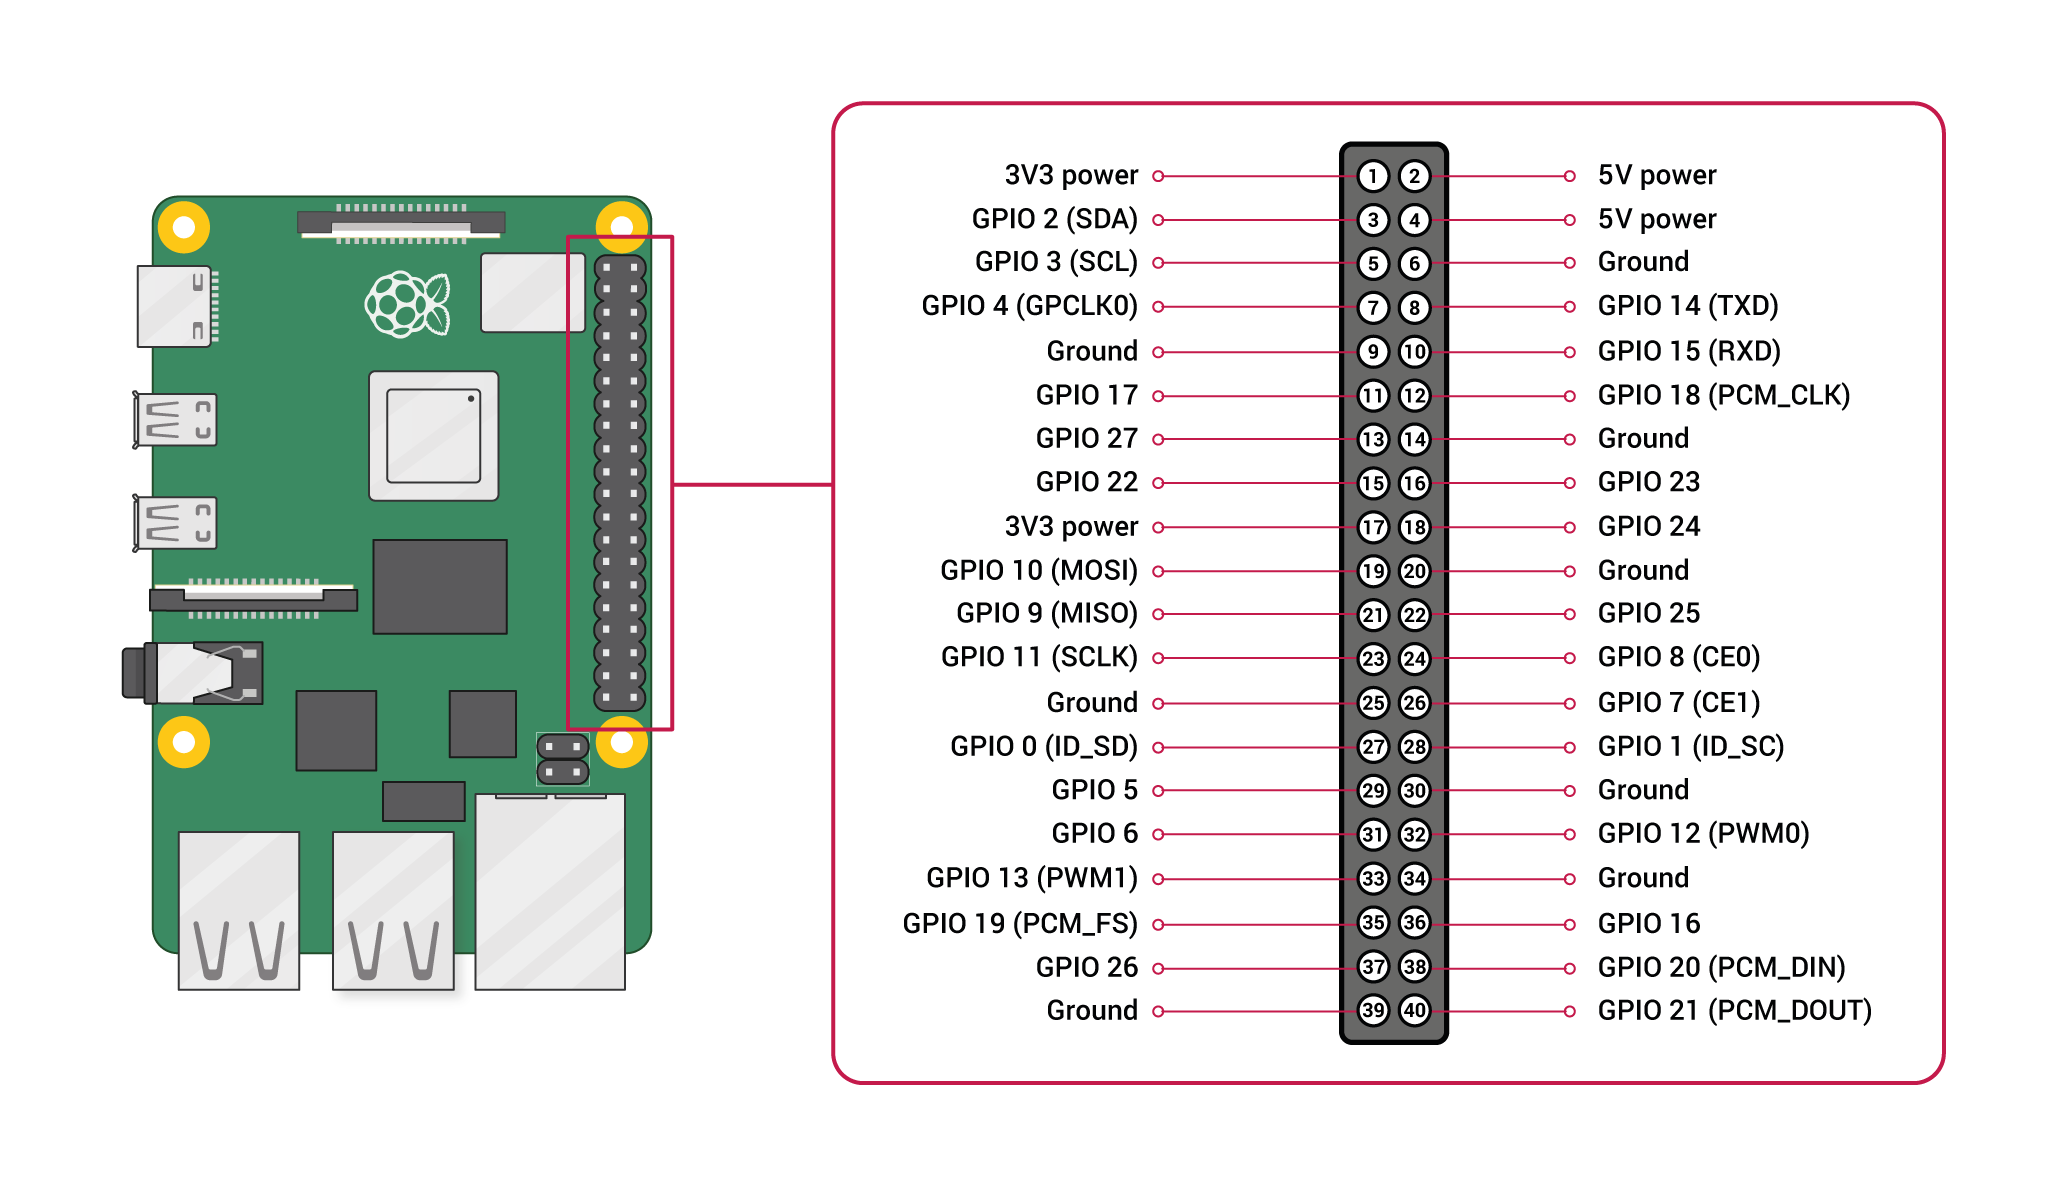
\includegraphics[width=0.5\textwidth]{figures/GPIO-Pinout-Diagram-2.png}
    \caption{\acrshort{gpio}s \textit{RaspberryPI} \cite{Raspberrytech}}
    \label{fig:gpio}
\end{figure}

A corrente no \gls{RaspberryPI} pode ser configurada para valores entre \SI{2}{\milli\ampere} e \SI{16}{\milli\ampere} (em intervalos de \SI{2}{\milli\ampere}) por cada \acrshort{gpio}. No entanto, quando vários \acrshort{gpio}s são utilizados em simultâneo, o valor total combinado da corrente não deve exceder os \SI{50}{\milli\ampere}. Se for fornecida uma tensão superior a \SI{3.3}{\volt} aos \acrshort{gpio}s, o \gls{RaspberryPI} corre o risco de se danificar irremediavelmente. \cite{Raspberrytech}. Na Figura \ref{fig:gpiocores} está representada uma forma alternativa de visualizar os \acrshort{gpio}s, mais intuitiva e que permite perceber melhor a função dos pinos. Representados a cor amarela estão os \acrshort{gpio}s que podem ser configurados como entrada ou saída; a vermelho, laranja e preto as alimentações de \SI{5}{\volt}, \SI{3.3}{\volt} e \textit{ground}, respectivamentee. Por fim, os \acrshort{gpio}s representados pela cor branca, \acrshort{gpio}0  e \acrshort{gpio}1, correspondentes aos pinos físicos 27 e 28, respectivamente, estão reservados para utilização avançada, nomeadamente, a comunicação \acrshort{i2c} com a \gls{eeprom} de identificação presente em \gls{hat}s compatíveis. Esta \gls{eeprom} permite a configuração automática do sistema aquando do arranque. 

\begin{figure}[hbtp]
    \centering
    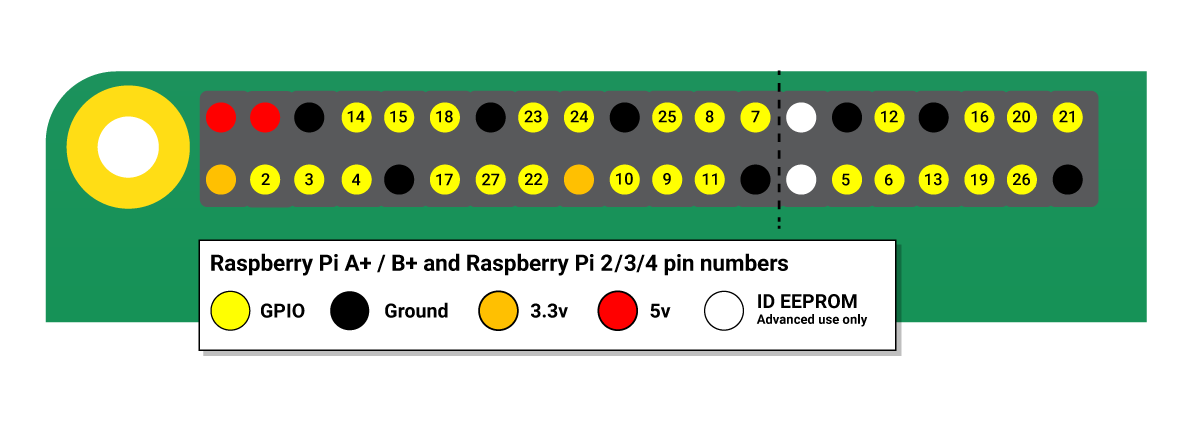
\includegraphics[width=0.5\textwidth]{figures/GPIO.png}
    \caption{Representação alternativa dos \acrshort{gpio}s \cite{Raspberrytech}}
    \label{fig:gpiocores}
\end{figure}

\subsection{Relés}
\label{sec:reles}
Como já foi referido na Capítulo \ref{Capitulo2}, os circuitos que compõem o \acrshort{visir} são controlados através de relés. Estes dispositivos funcionam como interruptores electromecânicos simples que utilizam um sinal elétrico para controlar um eletroíman.
Os relés electromecânicos são constituídos por uma bobine e um contacto, que pode ser normalmente aberto ou fechado. A corrente eléctrica ao passar pela bobine gera um campo magnético que atrai o contacto, fechando-o ou abrindo-o, conforme o caso. A Figura \ref{fig:esquematicoreles} mostra um esquema simplificado de um relé electromecânico, onde se pode observar a inclusão do díodo de ``roda livre'', comum em muitos circuitos de comando com relés. Este díodo é utilizado para proteger o circuito de comando de picos de tensão induzidos pela bobine do relé, quando a corrente é desligada, segundo a Lei de Faraday. O díodo permite que a corrente induzida pela bobine circule em circuito fechado, evitando danos nos componentes de comando. 

\begin{figure}[hbtp]
    \centering
    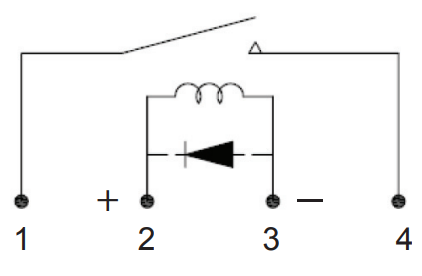
\includegraphics[width=0.3\textwidth]{figures/esquematico_rele.png}
    \caption{\textit{Esquema simplificado de um relé \cite{DryRelay}}}
    \label{fig:esquematicoreles}
\end{figure}

Os relés utilizados no \acrshort{lare} estavam disponíveis em contexto laboratorial e são em tudo idênticos aos que se encontram instalados no \acrshort{visir}  do \acrshort{isep}. Foram usados dois tipos de relés: simples (\acrfull{spst}) e duplos (\acrfull{dpst}), como ilustrado na Figura \ref {fig:reles}. Ambos os modelos são da marca \textit{Comus} - o relé \acrshort{spst}, ref. 3570-1331-123 e o relé \acrshort{dpst}, ref. 3572-1220-123. As características principais encontram-se descritas no Anexo~\ref{AppendixA} e as completas nos respectivos \textit{datasheet} \cite{DryRelay}. 

Nos códigos de referência dos relés, os dois primeiros quartetos indicam a série, enquanto os três dígitos indicam a tensão nominal da bobine e a presença, ou não, do díodo de ``roda livre''. No caso dos modelos utilizados, esta tensão é de \SI{12}{\volt} e o díodo está ligado entre os pinos 2(+) e 6(-) \cite{DryRelay}. Sempre que possível, tentou-se utilizar os relés \acrshort{spst} no comando das fontes e aparelhos de medida e os relés \acrshort{dpst} no controlo dos componentes. Serão devidamente referidos os casos em que isso não foi possível, por indisponibilidade dos componentes.

\begin{figure}[hbtp]
    \centering
    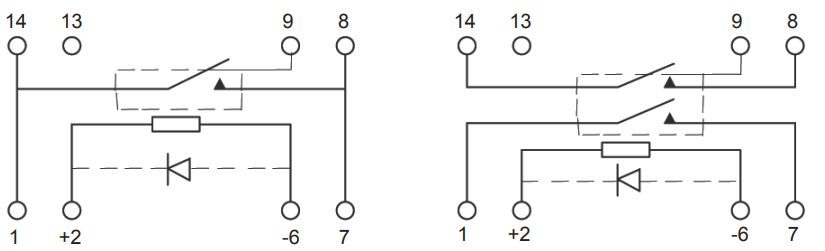
\includegraphics[width=0.5\textwidth]{figures/reles.png}
    \caption{\textit{Relés \acrshort{spst} e \acrshort{dpst}} \cite{DryRelay}}
    \label{fig:reles}
\end{figure}

Como já foi referido na Secção \ref{sec:RaspberryPI}, a tensão de funcionamento dos \acrshort{gpio}s, quer estejam configurados como entrada ou saída, é de \SI{3.3}{\volt}, sendo que a máxima corrente por cada \acrshort{gpio} é de \SI{16}{\mA}.
Com estes valores, o \gls{RaspberryPI} não tem capacidade para comandar os relés, já que funcionam a \SI{12}{\volt}. Para activar os relés, é necessário o uso de \textit{drivers}\footnote{Doravante, sempre que for referido o termo \textit{driver} no contexto de relés, subentende-se o circuito integrado \textit{ULN2003A}.} que consigam fornecer a tensão e corrente necessárias para o efeito.

\subsection{\textit{Driver} de Relés}
\label{sec:driver}
O circuito integrado ULN2003A, é um \textit{driver} muito usado para controlar relés. Além disso estava disponível em contexto laboratorial. Tipicamente, é usado em conjunto com microcontroladores ou \gls{RaspberryPI}\footnote{Importa distinguir entre \gls{sbc}s, como o \gls{RaspberryPI} e microcontroladores, como o Arduino. Enquanto os \gls{sbc}s funcionam como computadores completos capazes de executar sistemas operativos e aplicações complexas, os microcontroladores são dispositivos mais simples, ideais para tarefas de controlo directo, operando sem sistema operativo e com recursos significativamente mais limitados.} no comando de cargas indutivas, como motores, bobines e relés. Estes \textit{drivers} possuem sete pares de transístores NPN, em configuração \textit{Darlington}, que apresentam saídas de alta tensão com díodos \textit{clamp} de cátodo comum para comutação de cargas indutivas \cite{ULN2003}, como se  representa esquematicamente na Figura \ref{fig:2003blocos}.

\begin{figure}[hbtp]
    \centering
    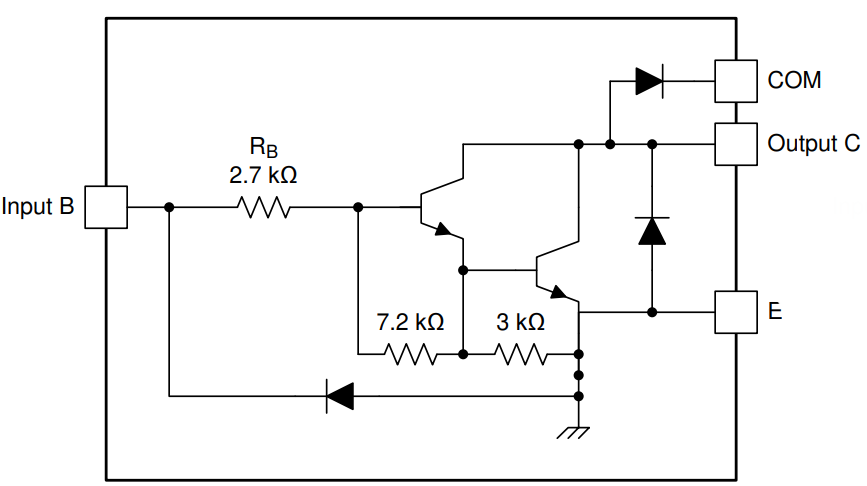
\includegraphics[width=0.5\textwidth]{figures/2003A_Darling.png}
    \caption{Diagrama de blocos ULN2003A \cite{ULN2003}}
    \label{fig:2003blocos}
\end{figure}

A corrente de colector de saída (única) é de \SI{500}{\mA} e a corrente de entrada, para uma tensão de entrada de \SI{3.85}{\volt}, é \SI{0.93}{\mA} \cite{ULN2003}.

Pela análise dos esquemas, representados no Anexo \ref{AppendixA} e já referenciado na Secção \ref{sec:matriz}, verifica-se que os \acrshort{gpio}s disponíveis no \gls{RaspberryPI} - 26 no total - não são suficientes para comandar os relés do \acrshort{lare}. Ao todo são utilizados 21 relés, o que corresponderia a 21 saídas, faltando adicionar 10 \acrshort{gpio}s necessários para o controlo da transmissão das \textit{strings} de \textit{bits}. Sendo assim, houve a necessidade de criar uma solução que permitisse comandar os relés, já que o \gls{RaspberryPI} não possui \acrshort{gpio}s suficientes.

\subsection{Registo de deslocamento}
\label{sec:registodeslocamento}
O uso de registos de deslocamento foi a solução encontrada de forma a ultrapassar o problema da falta de \acrshort{gpio}s. O \textit{SN74HC595}\footnote{Doravante, sempre que for referido registo de deslocamento, subentende-se o circuito integrado \textit{SN74HC595}.} é um circuito integrado comum e bastante utilizado que contém um registo de deslocamento de 8 \textit{bits} com saídas \textit{3-State}, do tipo \acrfull{sipo}, que alimenta um registo de armazenamento do tipo D, também de 8 \textit{bits} e com saídas paralelas \textit{3-State}. O sinal de relógio para o registo de deslocamento e armazenamento é independente. A potência consumida é muito baixa, assim como a corrente de entrada \cite{SN74HC595}.

Descrição dos pinos de controlo:
\begin{itemize}
    \item \acrfull{ser}: é utilizado para enviar os \textit{bits} para o registo de deslocamento, um \textit{bit} de cada vez;

    \item \acrfull{srclk}: é o relógio do registo de deslocamento e é ativado no flanco ascendente, por cada impulso dado um \textit{bit} é enviado para o registo de deslocamento;

    \item \acrfull{rclk}: é o relógio do do registo de armazenamento e é activo no flanco ascendente. Quando activo, o conteúdo do registo de deslocamento é transferido para o registo de armazenamento, que eventualmente aparece na saída;

    \item \acrfull{srclr}: permite fazer o \textit{clear} ou \textit{reset} ao registo de deslocamento. Isto equivale a colocar todos os \textit{bits} a zero. Este pino é activo baixo.

    \item \acrfull{oe}: pino activo baixo que controla o estado da saída do registo: Se a zero as saídas estão activas, se a um as saídas estão desactivadas
\end{itemize}

Como referido na Secção~\ref{sec:matriz}, a experiência da Lei de \textit{Ohm} requer 8 relés, enquanto as experiências de rectificadores e filtros necessitam de 13. Cada relé é acionado por um \textit{bit} de um registo de deslocamento, sendo que cada registo permite o controlo de até 8 relés. Assim, é necessário um registo para a experiência da Lei de \textit{Ohm} e dois registos para as experiências de rectificação e filtragem.
Deste modo, é enviada uma \textit{string} de 8 ou 13 \textit{bits}, conforme a experiência a controlar - os \textit{bits} são enviados um-a-um, armazenados no registo e depois enviados para a saída. Dado que o número de \textit{bits} varia entre experiências e estas se encontram distribuídas por duas placas distintas (conforme descrito na Secção~\ref{sec:matriz}), optou-se por utilizar pinos diferentes do \gls{RaspberryPI} para o envio das \textit{strings}. No Anexo \ref{AppendixA}, Figura 11 e Figura 12, estão definidos os pinos usados na configuração e envio das \textit{strings}. A Figura~\ref{fig:SN74HC595blocos} apresenta o diagrama de blocos do registo de deslocamento, enquanto a Tabela~\ref{Table:funcSN74HC595} descreve os seus modos de funcionamento. Como se pode observar, o controlo do envio de uma \textit{string} de dados requer 5 pinos \acrshort{gpio} configurados como saídas. Deste modo, para comandar os relés das experiências distribuídas pelas duas placas, são necessários 10 pinos \acrshort{gpio} no total.

\begin{figure}[hbtp]
    \centering
    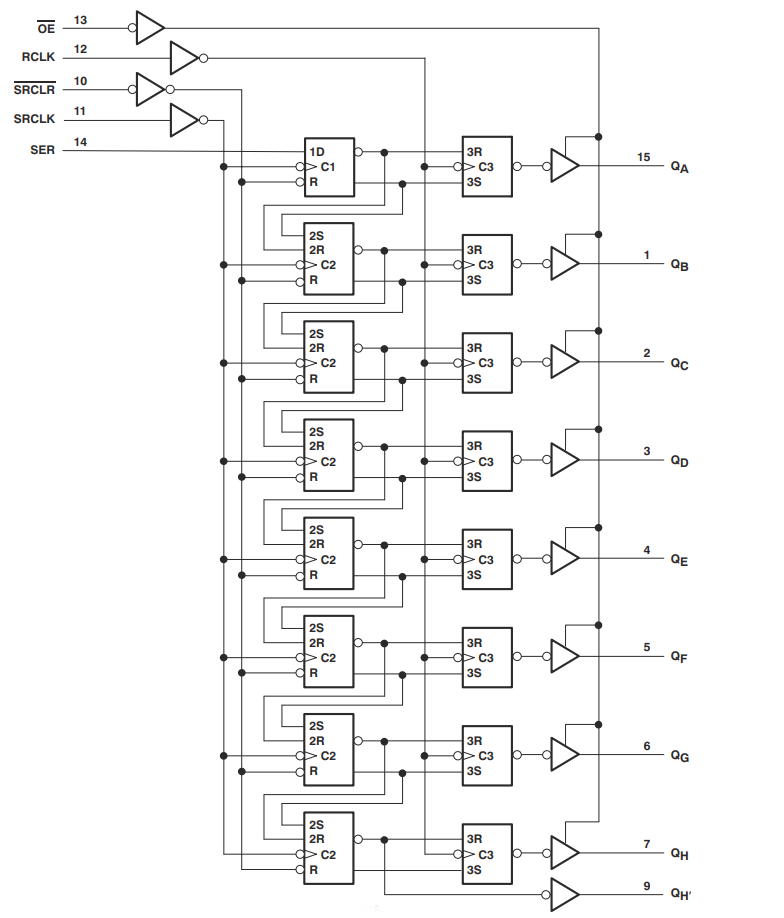
\includegraphics[width=0.7\textwidth]{figures/SR_blocos.png}
    \caption{Diagrama \textins{em corte} de blocos SN74HC595 \cite{SN74HC595}}
    \label{fig:SN74HC595blocos}
\end{figure}

Importa notar que seria tecnicamente possível reduzir este número para apenas 6 pinos, utilizando os mesmos sinais de controlo para ambos os registos de deslocamento e activando-os seletivamente através da linha \textit{OE - Output Enable} de cada registo. No entanto, dado que a implementação e os testes dos circuitos foram realizados de forma faseada, optou-se por manter conjuntos de pinos independentes para cada registo de deslocamento, facilitando a deteção e resolução de eventuais erros. As implicações ao nível do \textit{software} de programação são mínimas e ao nível do \textit{hardware} estão dentro dos limites de número de \acrshort{gpio}s do \gls{RaspberryPI}.

\begin{table}[htb]
    \caption{Modos de funcionamento do SN74HC595 \cite{SN74HC595}}
    \label{Table:funcSN74HC595}
    \resizebox{\textwidth}{!}{%
        \begin{tabular}{cccccl}
            \toprule
            \multicolumn{5}{c}{Entradas}           & \multicolumn{1}{c}{\multirow{3}{*}{Função}}                                                                                        \\
            \cline {1-5}
            \multicolumn{5}{l}{}                   &
            \multicolumn{1}{c}{}                                                                                                                                                        \\
            \multicolumn{1}{l}{SER}                &
            \multicolumn{1}{l}{SRCLK}              &
            \multicolumn{1}{l}{$\overline{SRCLR}$} &
            \multicolumn{1}{l}{RCLK}               &
            \multicolumn{1}{l}{$\overline{OE}$}    &
            \multicolumn{1}{c}{}                                                                                                                                                        \\
            \midrule
            X                                      & X                                           & X & X          & H & Saídas $Q_A$ - $Q_H$ estão desabilitadas.                       \\
            \midrule
            X                                      & X                                           & X & X          & L & Saídas $Q_A$ - $Q_H$ estão habilitadas.                         \\
            \midrule
            X                                      & X                                           & L & X          & X & Registo de deslocamento é limpo.                                \\
            \midrule
            L                                      &
            $\uparrow$                             &
            H                                      &
            X                                      &
            X                                      &
            \begin{tabular}[c]{@{}l@{}} Primeiro passo do registo de deslocamento vai a ``0''. \\ Passo seguinte armazena os dados do estado anterior, respectivamente. \end{tabular}   \\
            \midrule
            H                                      &
            $\uparrow$                             &
            H                                      &
            X                                      &
            X                                      &
            \begin{tabular}[c]{@{}l@{}}Primeiro passo do registo de deslocamento vai a ``1''. \\ Passo seguinte armazena os dados do estado anterior, respectivamente. \end{tabular}    \\
            \midrule
            X                                      & X                                           & X & $\uparrow$ & X & Os dados do registo de deslocamento são armazenados no registo. \\
            \bottomrule
        \end{tabular}%
    }
\end{table}

\section{Software}
\label{sec:arquitecturasoftware} 
O \textit{software} do \acrshort{lare} foi dividido em duas grandes partes: \textit{Back-end} e \textit{Front-end}.

Por \textit{Back-end} entende-se toda a programação e os processos que correm em segundo plano w que sustentam o funcionamento do \acrshort{lare}, incluindo o servidor, as \acrshort{api}s ou base de dados \cite{FrontbackEnd}. Existem diversas linguagens de programação, \textit{frameworks} e ferramentas para gerir esta parte do sistema. Na implementação do \acrshort{lare}, foi utilizada a linguagem \textit{Python}, em conjunto com a \textit{Framework} \textit{Flask} .

O \textit{Front-end}, por sua vez, gere a \textit{interface} do \textit{site}, ou seja, a camada com que o utilizador interage directamente. As linguagens utilizadas na sua implementação foram o \acrshort{html}, \acrfull{css} e \textit{JavaScript}. Enquanto o \acrshort{html} constitui a estrutura base da página, o \acrshort{css} define o estilo visual dos elementos o \textit{JavaScript} permite a criação de comportamentos dinâmicos e interactivos \cite{FrontbackEnd}.

De forma resumida, o desenvolvimento de \textit{Front-end} corresponde ao lado do cliente (aspecto da página \textit{Web}), enquanto o \textit{Back-end} diz respeito ao lado do servidor (funcionamento da página \textit{Web}).

\subsection{\textit{Back-End}}
\label{sec:back-end}
\subsubsection{\textit{Python}}
O \textit{Python} é uma linguagem poderosa e fácil de aprender. Possui estruturas de dados de alto nível eficientes e uma abordagem simples, mas eficaz à programação orientada para objectos \cite{ThePython}. Apresenta, também, uma série de vantagens que se enquadram nos objectivos do desenvolvimento e implementação do \acrshort{lare} \cite{pythonvantagens}:
\begin{itemize}
    \item Curva suave de aprendizagem;
    \item Quantidade e variedade das bibliotecas;
    \item Portabilidade;
    \item Flexibilidade;
    \item Robustez;
    \item Suporte da comunidade.
\end{itemize}

Como desvantagens há a referir que, comparado com outras linguagens, o \textit{Python} é mais lento em termos de execução, já que é um tipo de linguagem de alto-nível, pelo que não é adaptado para aplicações móveis e consome mais recursos \cite{pythonvantagens} \cite{5MainDispython}. Ainda assim, segundo a \textit{IEEE Spectrum} \cite{ieeespectrum}, a linguagem \textit{Python} foi considerada a mais popular em 2023.

\subsubsection{\textit{Flask}}
O \textit{Flask} é uma \textit{framework} leve e flexível para \textit{Python} que segue a filosofia \textit{UNIX} de ``fazer uma coisa bem feita''. A escolha do \textit{Flask} deveu-se, essencialmente, à facilidade de integração com o \textit{Python}, sendo uma das \textit{frameworks} mais populares em \textit{Python} \cite{Flask}. É uma \textit{framework} de aplicações \acrfull{wsgi} que descreve a forma como um servidor \textit{Web} comunica com aplicações \textit{Web} e como essas aplicações podem ser encadeadas para processar um pedido \cite{wsgi}. Depende, ainda do  \textit{Jinja}, que é um motor de criação de modelos que permite escrever código semelhante à sintaxe do \textit{Python}, de forma a renderizar o documento final \cite{Jinja}.

Tal como foi referido na Secção \ref{sec:contextualização}, foram ainda analisadas várias opções, incluindo a \textit{Django}, outra \textit{framework} bastante popular. Em \cite{Djangovsflask} e \cite{FlaskvsDjango}, por exemplo, é feita uma comparação exaustiva entre as duas \textit{frameworks}, não havendo uma decisão final sobre qual a melhor, mas sim sobre qual a que melhor se adapta às necessidades de implementação e desenvolvimento dos projectos. No entanto, o \textit{Flask} foi concebido para tornar a iniciação rápida e fácil, com a capacidade de evoluir até aplicações mais complexas, sendo mais adapatado a pequenos projectos.

Tendo em conta os argumentos anteriormente apresentados e a análise dos respetivos prós e contras, considerou-se que a linguagem de programação \textit{Python}, em conjugação com o \textit{Flask} enquanto \textit{framework} para desenvolvimento de aplicações web e APIs, constitui a solução que melhor se enquadra e adapta aos objectivos definidos para o \acrshort{lare}.

\subsubsection{\textit{Jinja2}}
\label{sec:jinja2}
O \textit{Jinja2}\footnote{O nome \textit{Jinja2} refere-se à versão actual do sistema de \textit{templates} Jinja, resultante de uma reescrita significativa da sua versão original. Na documentação e na comunidade, é comum referir-se a este motor simplesmente como \textit{Jinja} \cite{Jinja}. Assim, e sem perda de generalidade, será adoptada ao longo deste trabalho a designação \textit{Jinja}.} é um sistema de \textit{templates} para aplicações \textit{Web} escrito em \textit{Python}, amplamente utilizado em conjunto com a \textit{framework} \textit{Flask}. O seu principal objetivo é permitir a separação entre a lógica da aplicação e a apresentação visual, promovendo um desenvolvimento mais organizado, modular e sustentável. Inspirado na sintaxe do próprio \textit{Python}, o \textit{Jinja} permite incorporar estruturas de controlo, como ciclos e condições, diretamente nos ficheiros \acrshort{html} através de marcação específica, facilitando a criação dinâmica de conteúdo \cite{Jinja}. Na Listagem \ref{lst:exemplojinja} pode ver-se um exemplo de código \textit{Jinja} incluído na página \textit{base.html}.

\begin{minipage}{0.9\linewidth}
    \begin{lstlisting}[language=python, caption=Exemplo \textit{Jinja} incluído na página \textit{base.html}, label=lst:exemplojinja]
	<title>Home</title>
    
        <a class="nav-item nav-link" id="home" href="/">Home</a>
    
        <a class="nav-item nav-link" id="login" href="/login">Login</a>
    

    
    
        {{ message }}
    
    

	\end{lstlisting}
\end{minipage}

O mecanismo de \textit{renderização} disponibilizado pelo \textit{Flask}, através da função \textit{render\_template()}, tira partido do \textit{Jinja} para gerar páginas \acrshort{html} com base em \textit{templates} pré-definidos e dados fornecidos pela aplicação. Isto permite, por exemplo, apresentar resultados de medições, estado dos relés ou mensagens personalizadas, de forma automatizada e responsiva. O \textit{Jinja2} permite gerar \acrshort{html} dinâmico através da substituição de variáveis $(\{\{ \ldots \}\})$ e da execução de instruções lógicas ({\% \ldots \%}) no lado do servidor, antes de o conteúdo ser enviado ao navegador. Como resultado, o utilizador final visualiza apenas o \acrshort{html} já processado, sem qualquer traço do código \textit{Jinja}. Esta abordagem estabelece uma ligação simples e segura entre a lógica implementada em \textit{Python} no \textit{back-end} e a apresentação em \acrshort{html} no \textit{front-end} \cite{Jinja}. 

\subsection{Front-End}
\label{sec:frontend}
\subsubsection{\textit{Webpage}}
Como já foi referido na Secção \ref{sec:arquitecturasoftware}, o \textit{Front-end} diz respeito ao aspecto gráfico das páginas \textit{Web} e pretende-se que a prioridade na construção da página seja a simplicidade. A escolha do desenvolvimento da página recaiu no \acrshort{html}, \acrshort{css} e \textit{JavaScript}.

O \acrshort{html} é a linguagem \textit{standard}, usada para definir a estrutura do seu conteúdo e consiste numa série de elementos usados para delimitar ou agrupar diferentes partes do conteúdo. As \textit{tags} ou etiquetas, podem transformar uma palavra ou imagem num \textit{hyperlink}, pôr palavras em itálico, aumentar ou diminuir a fonte, etc. \cite{HTMLbasics}

Existem 3 tipos de elementos \cite{HTMLwikipedia}:
\begin{itemize}
    \item \textbf{Normais}: são elementos que têm uma etiqueta de abertura e outra de fecho. Por exemplo, <p></p> define um parágrafo;
    \item \textbf{Texto}: são elementos que não têm uma etiqueta de fecho. Por exemplo, <Title> especifica o título da página em texto simples;
    \item \textbf{Vazios}: têm somente uma etiqueta de início na forma de <tag>. Por exemplo, a etiqueta <img> referencia um ficheiro externo, neste caso uma imagem ou <br> que força uma quebra de linha.
\end{itemize}

Na Figura \ref{fig:estruturahtml} está representada a estrutura de uma página \acrshort{html}. De referir os navegadores não exibem as etiquetas HTML. O seu propósito é ler os documentos \acrshort{html} e apresentá-los corretamente.

\begin{figure}[hbtp]
    \centering
    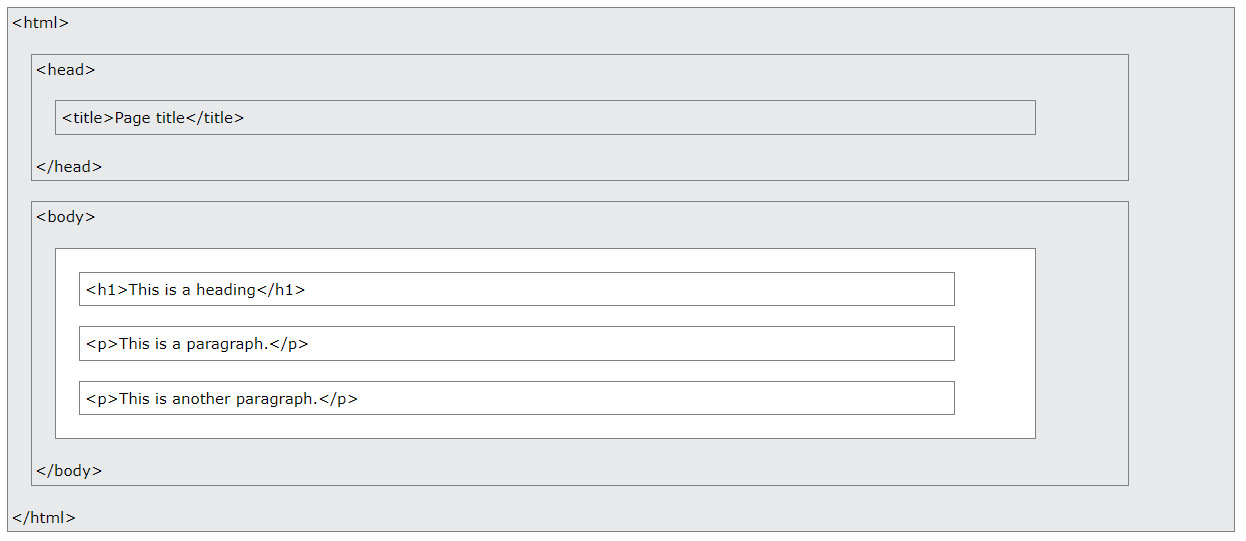
\includegraphics[width=0.7\textwidth]{figures/html_page_structure.png}
    \caption{Estrutura de uma página \acrshort{html} \cite{HTMLbasics}}
    \label{fig:estruturahtml}
\end{figure}

Segundo o consórcio \gls{w3c}, as \acrshort{css} são mecanismos fundamentais para a separação de preocupações no desenvolvimento \textit{web}. Ao delegar a responsabilidade de formatação visual no \acrshort{css}, o \acrshort{html} concentra-se na estrutura semântica do conteúdo. Isso resulta num código mais limpo, de fácil manutenção e acessível. As regras de estilo, que especificam como os elementos \acrshort{html} devem ser apresentados, podem ser aplicadas a elementos individuais, classes ou \textit{IDs}, permitindo um alto grau de customização. Além disso, o \acrshort{css} oferece a possibilidade de criar hierarquias de estilos, onde os mais específicos sobrepõem aos mais gerais. As folhas de estilo podem ser inseridas diretamente no documento \acrshort{html} ou vinculadas a ele através de um arquivo externo, proporcionando maior organização e reutilização de estilos \cite{w3ccss}. Um exemplo simples pode ser visto na Listagem \ref{lst:excss}.

\begin{minipage}{0.9\linewidth}
    \begin{lstlisting}[language=HTML, caption=Exemplo \acrshort{css} incluído na página \acrshort{html} \cite{Startingcss}, label=lst:excss]
		<!DOCTYPE html PUBLIC "-//W3C//DTD HTML 4.01//EN">
		<html>
		<head>
		  <title>My first styled page</title>
		  <style type="text/css">
		  body {
			color: purple;
			background-color: #d8da3d }
		  </style>
		</head>
		
		<body>
		(...)
	\end{lstlisting}
\end{minipage}

As linhas 5 e 6 indicam que é uma folha de estilos escrita em \acrshort{css} e que o estilo está aplicado ao elemento \textit{body}. As linhas seguintes definem as cores do texto e fundo. No exemplo dado na Listagem \ref{lst:excss}, a folha de estilos está integrada directamente no ficheiro \acrshort{html}. Mas à medida que a página cresce em complexidade, torna-se incomportável manter a folha de estilos no ficheiro (ou ficheiros) \acrshort{html}. Para isso, cria-se a folha de estilos com a extensão \textit{.css} e referencia-se este ficheiro em todas as páginas. Neste caso, o exemplo da página apresentado na Listagem \ref{lst:excss} ficaria da forma apresentada na Listagem \ref{lst:paginahtmlcss}:

\begin{minipage}{0.9\linewidth}
    \begin{lstlisting}[language=HTML, caption=Exemplo da página \acrshort{html} com o \acrshort{css} definida externamente \cite{Startingcss}, label=lst:paginahtmlcss]
		<!DOCTYPE html PUBLIC "-//W3C//DTD HTML 4.01//EN">
		<html>
		<head>
		  <title>My first styled page</title>
		  <link rel="stylesheet" href="meuestilo.css">
		</head>
		
		<body>
		(...)
	\end{lstlisting}
\end{minipage}

Por sua vez, o ficheiro \textit{\textbf{meuestilo.css}} da forma apresentada na Listagem \ref{lst:cssexterno}:

\begin{minipage}{0.9\linewidth}
    \begin{lstlisting}[language=HTML, caption=Exemplo do \acrshort{css} definido externamente \cite{Startingcss}, label=lst:cssexterno]
		body {
			color: purple;
			background-color: #d8da3d }
		  </style>
		(...)
	\end{lstlisting}
\end{minipage}

As folhas de estilo \acrshort{css} e as páginas \acrshort{html} podem ser validadas para garantir que estão de acordo com os padrões definidos pelo consórcio \gls{w3c} \cite{cssvalidator, htmlvalidator}. Esta validação é importante para assegurar a compatibilidade entre navegadores e dispositivos, bem como para melhorar a acessibilidade e a experiência do utilizador.

Já o \textit{JavaScript} é uma linguagem de programação orientada para objectos e utilizada principalmente para \textit{scripts} dinâmicos do lado do cliente, permitindo que uma aplicação coloque elementos num formulário \acrshort{html} e responda a eventos do utilizador, como cliques do rato, preenchimento de formulários e navegação na página. Também pode ser utilizada no lado do servidor, permitindo que uma aplicação comunique com uma base de dados, mantenha a continuidade das informações entre diferentes chamadas da aplicação ou manipule ficheiro no servidor. Isso significa que, no navegador, o \textit{JavaScript} pode alterar a aparência da página e, da mesma forma, o \textit{Node.js} - versão mais avançada do \textit{JavaScript} no servidor - pode responder a solicitações personalizadas enviadas pelo código executado no navegador.  Os programas escritos nesta linguagem são designados por \textit{scripts} e podem ser inseridos diretamente numa página \acrshort{html}, sendo executados automaticamente aquando do seu carregamento. Por serem interpretados, estes scripts são escritos em texto simples e não requerem compilação prévia para serem executados. O JavaScript pode ser executado não apenas nos navegadores, mas também nos servidores, ou, basicamente, em qualquer dispositivo que tenha um \textit{JavaScript Engine}, isto é, \textit{software} específico que execute o código \textit{JavaScript} \cite{JavaScriptRef}. Na Listagem \ref{lst:exemplojava} está representado um exemplo de \textit{JavaScript} que desabilita os seletores de um formulário quando o botão ``OK'' é clicado.

\begin{minipage}{0.9\linewidth}
    \begin{lstlisting}[language=HTML, caption=Exemplo de \textit{JavaScript}, label=lst:exemplojava]
(...)
<script>
//Accionar a funcao habilitarSeletores quando o botao "OK" for clicado

document
  .querySelector(".stop")
  .addEventListener("click", desabilitarSeletores);
</script>
(...)
	\end{lstlisting}
\end{minipage}

Estas linguagens - \acrshort{html}, \acrshort{css} e \textit{JavaScript} - são interdependentes e frequentemente utilizadas em conjunto no desenvolvimento \textit{web}, cada uma desempenhando um papel específico na construção e estilização de páginas \textit{web} e na implementação de interatividade. Se o \acrshort{html} define o conteúdo das páginas, o \acrshort{css} define a sua aparência e o \textit{JavaScript} define o comportamento \cite{JavaScript}.


Apesar de a arquitectura modular permitir a futura adição de novos módulos e experiências, a actual implementação abrange apenas um conjunto básico. A expansibilidade do sistema está assegurada, mas levanta questões de ordem \textit{software} e/ou \textit{hardware}. Tal como está concebido, a \textit{string} de controlo utilizada para activar os relés varia consoante a experiência: no caso da Lei de \textit{Ohm}, é composta por 8 \textit{bits}; nas experiências de rectificação e filtragem, são necessários 13 \textit{bits}, correspondendo ao número de relés a comandar. No \acrshort{lare}, optou-se por utilizar um conjunto de cinco pinos de controlo dedicados por placa, como apresentado na Tabela~\ref{Table:funcSN74HC595}.